\chapter{Réalisation de l'application}
\section{Introduction}
Une fois la conception validée, nous sommes passés à la phase de développement. Cette section décrit les technologies choisies pour réaliser la plateforme, puis présente les principales interfaces de l'application.

\section{Outils et technologies utilisés}

\subsection{React}
\begin{figure}[H]
    \centering
    
\includegraphics[width=0.25\textwidth]{Logos/React logo.png}
    \caption{Logo de React}
\end{figure}
React est une bibliothèque JavaScript développée par Meta pour créer des interfaces utilisateur sous forme de composants réutilisables. Nous l'avons utilisé avec TypeScript pour le typage statique, ce qui facilite la maintenance du code et la détection d'erreurs.

\subsection{Vite}
\begin{figure}[H]
    \centering
    
\includegraphics[width=0.25\textwidth]{Logos/Vite logo.png}
    \caption{Logo de Vite}
\end{figure}
Vite est un outil de build moderne pour les applications web. Il offre un serveur de développement rapide avec du rechargement à chaud (Hot Module Replacement) et un bundling optimisé pour la production. Nous l'avons choisi pour sa rapidité par rapport à des alternatives comme Webpack.

\subsection{Tailwind CSS}
\begin{figure}[H]
    \centering
    
\includegraphics[width=0.25\textwidth]{Logos/Tailwind logo.png}
    \caption{Logo de Tailwind CSS}
\end{figure}
Tailwind CSS est un framework CSS utility-first qui permet de styliser les composants directement dans le code sans écrire de fichiers CSS séparés. Il accélère le développement et assure une cohérence visuelle sur toute l'application.

\subsection{Python}
\begin{figure}[H]
    \centering
    
\includegraphics[width=0.25\textwidth]{Logos/Python logo.png}
    \caption{Logo de Python}
\end{figure}
Python est le langage de programmation utilisé pour les deux backends de la plateforme. Sa syntaxe claire et son écosystème riche (Django, pandas, openpyxl) en font un choix adapté pour le développement d'API et le traitement de données.

\subsection{Django et Django REST Framework}
\begin{figure}[H]
    \centering
    
\includegraphics[width=0.25\textwidth]{Logos/Django logo.png}
    \caption{Logo de Django}
\end{figure}
Django est un framework web Python qui suit l'architecture MVT (Model-View-Template). Nous l'avons utilisé avec Django REST Framework (DRF) pour exposer des API REST consommées par le frontend React. La plateforme comporte deux backends Django : un pour O-PAGe et un pour M-PAGe.

\subsection{PostgreSQL}
\begin{figure}[H]
    \centering
    
\includegraphics[width=0.25\textwidth]{Logos/PostgreSQL Logo.png}
    \caption{Logo de PostgreSQL}
\end{figure}
PostgreSQL est le système de gestion de base de données relationnelle utilisé pour stocker l'ensemble des données de la plateforme (risques, indicateurs, piliers, campagnes, résultats). Les deux backends partagent la même base de données.

\subsection{Docker}
\begin{figure}[H]
    \centering
    
\includegraphics[width=0.25\textwidth]{Logos/Docker logo.png}
    \caption{Logo de Docker}
\end{figure}
Docker permet de conteneuriser chaque service de l'application (frontend, backend O-PAGe, backend M-PAGe, PostgreSQL, pgAdmin) dans des conteneurs isolés. Docker Compose coordonne l'ensemble de ces conteneurs en local et permet de lancer toute la plateforme sur une seule machine avec une seule commande : \texttt{docker compose up --build}.

\subsection{Git et GitHub}
\begin{figure}[H]
    \centering
    
\includegraphics[width=0.25\textwidth]{Logos/Github logo.png}
    \caption{Logo de GitHub}
\end{figure}
Git est utilisé pour le versioning du code. GitHub sert de plateforme de collaboration entre les membres de l'équipe : hébergement du dépôt, gestion des branches et suivi de l'avancement du projet.

\subsection{Récapitulatif des technologies}
Le tableau suivant résume les principales technologies et leur rôle dans le projet :

\begin{table}[H]
\centering
\renewcommand{\arraystretch}{1.3}
\begin{tabular}{@{}p{0.30\textwidth}p{0.62\textwidth}@{}}
\hline
\textbf{Technologie} & \textbf{Rôle} \\
\hline
React + TypeScript & Interface utilisateur (frontend) \\
\hline
Vite & Bundler et serveur de développement \\
\hline
Tailwind CSS & Style et mise en page \\
\hline
Python & Langage backend \\
\hline
Django + DRF & Framework backend et API REST \\
\hline
PostgreSQL & Base de données relationnelle \\
\hline
Docker & Conteneurisation et coordination locale \\
\hline
Git / GitHub & Versioning et collaboration \\
\hline
\end{tabular}
\caption{Technologies principales du projet}
\end{table}

\section{Réalisation de l'application web}
\subsection{Page d'authentification}
\begin{figure}[H]
    \centering
    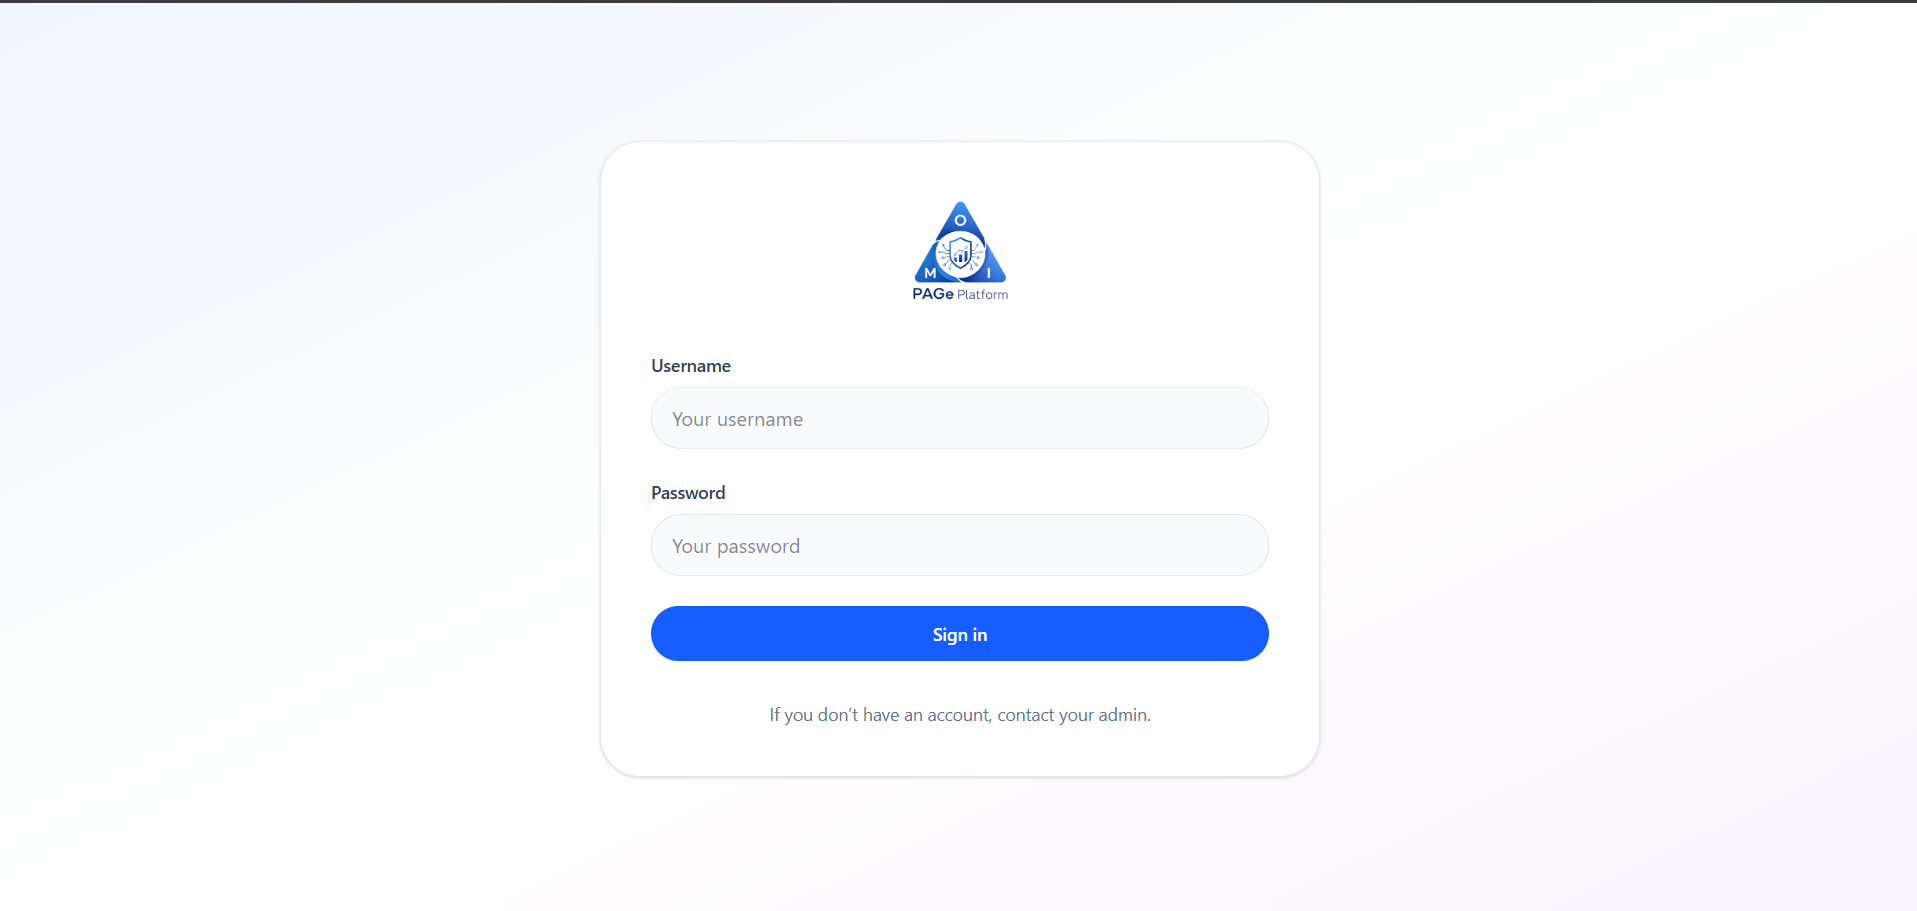
\includegraphics[width=0.8\textwidth]{Interfaces/Authentification.png}
    \caption{Interface d'authentification }
\end{figure}
L’interface d’authentification constitue le point d’entrée sécurisé de la plateforme PAGe. Elle dispose d'un formulaire épuré invitant l'utilisateur à saisir ses identifiants personnels afin de garantir la confidentialité et l'intégrité de l'accès au système. Cette interface redirige dynamiquement chaque profil connecté, qu’il s’agisse de l’Administrateur, de l'Organisateur, de l'Auditeur, du Décideur ou des Responsables, vers son propre espace de travail personnalisé.
\subsection{Page d'administration}
\begin{figure}[H]
    \centering
    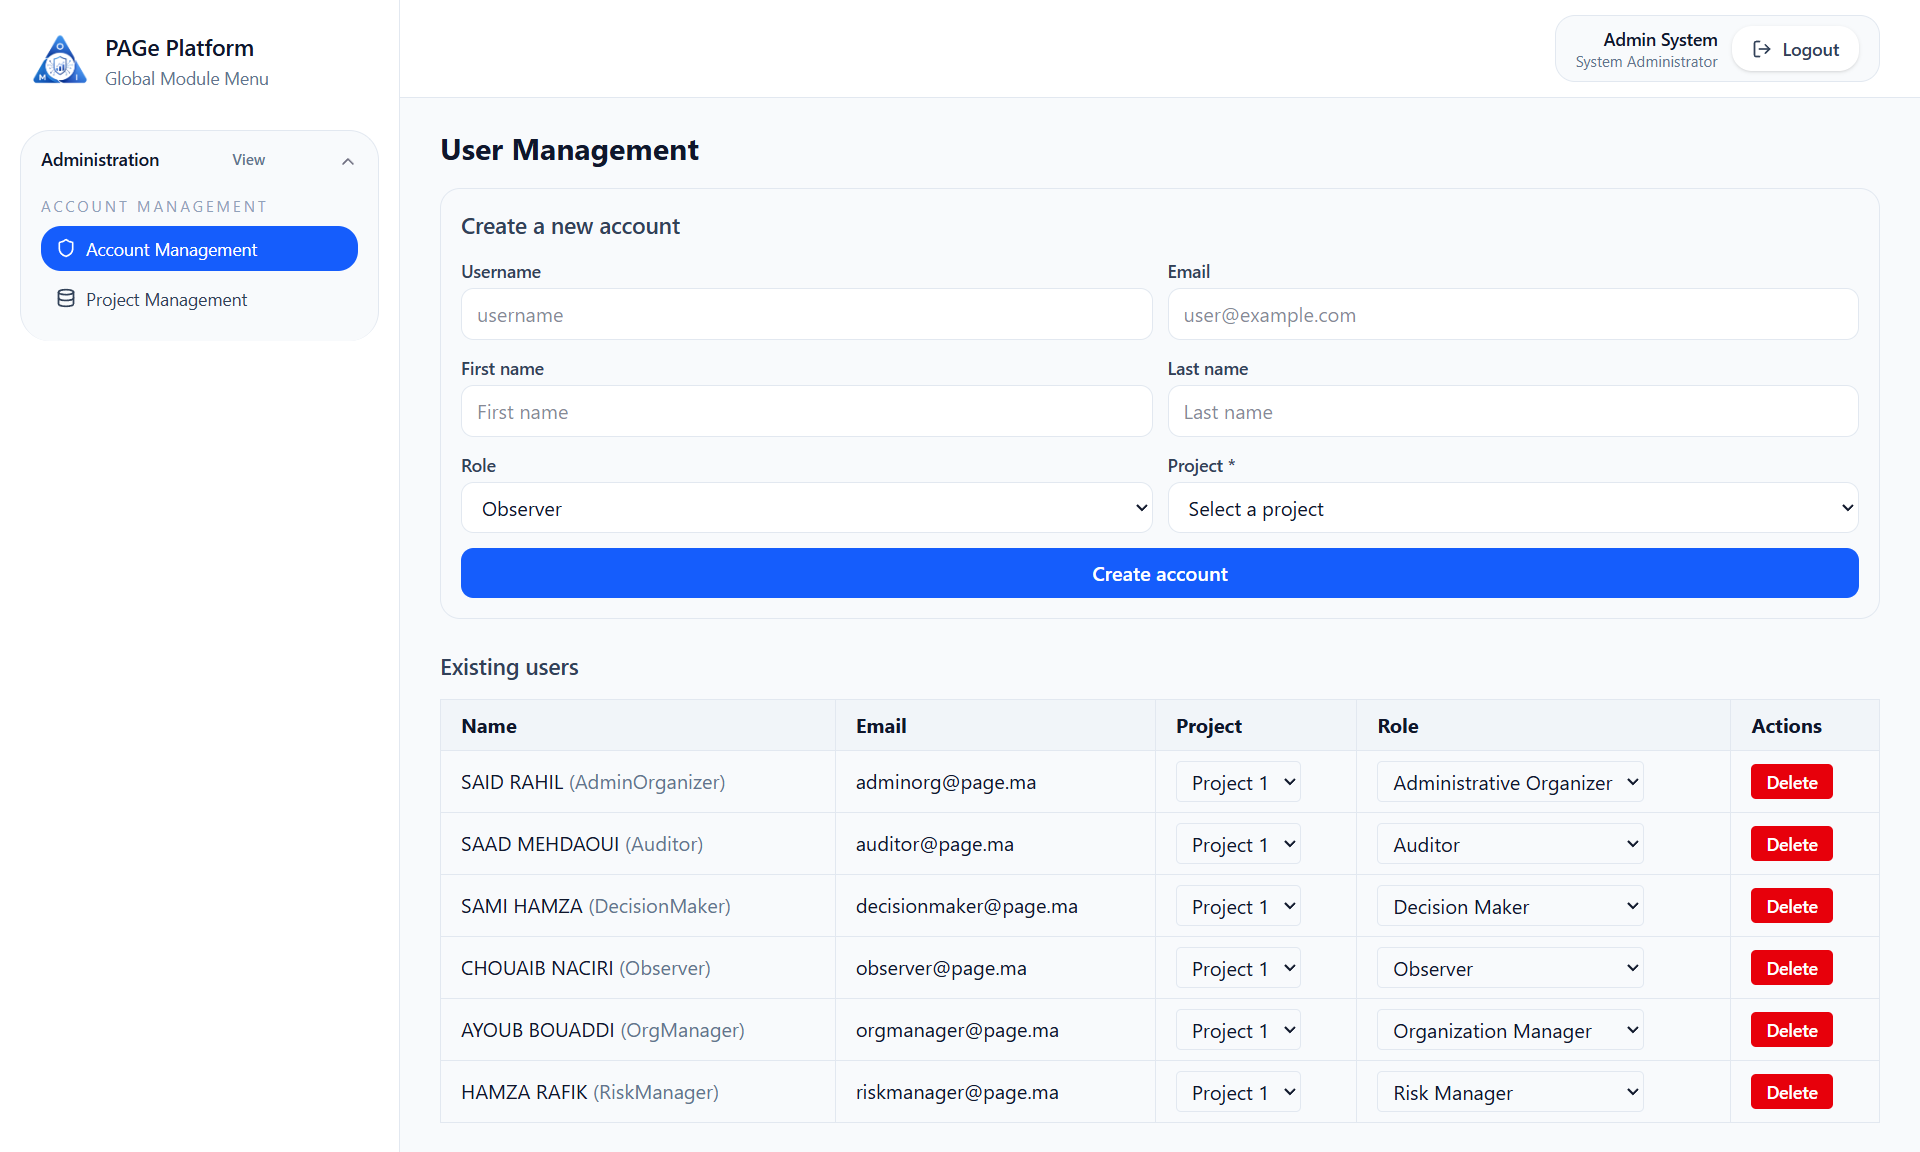
\includegraphics[width=0.7\textwidth]{Interfaces/Admin.png}
    \caption{Interface de gestion des utilisateurs }
\end{figure}
L'interface d'administration est dédiée à la gestion globale de la sécurité et des comptes utilisateurs. Elle offre un formulaire de création permettant à l'administrateur système d'enregistrer de nouveaux profils en renseignant leurs informations personnelles et en leur assignant un projet ainsi qu'un rôle spécifique parmi ceux prévus (Observateur, Auditeur, Décideur, etc.).
\subsection{Page des projets}
\begin{figure}[H]
    \centering
    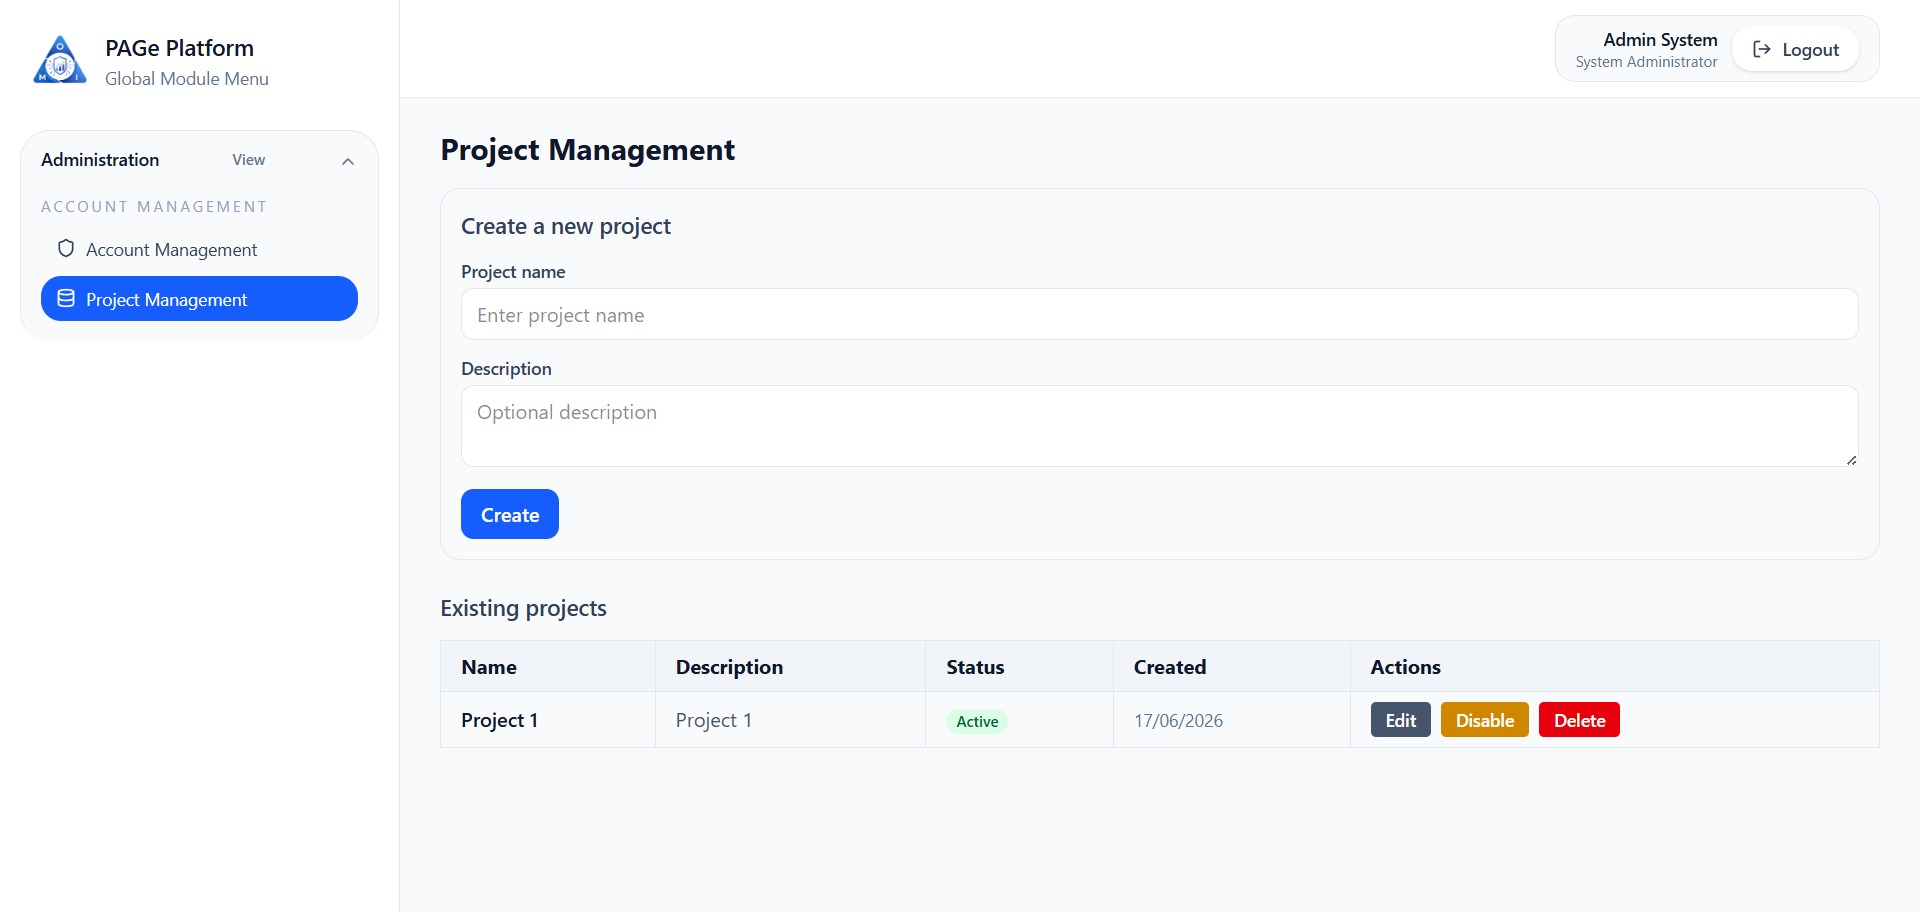
\includegraphics[width=0.8\textwidth]{Interfaces/Creation Project.png}
    \caption{Interface de gestion des projets }
\end{figure}
L'interface de gestion de projets permet à l'administrateur d'initialiser et de configurer les différents projets de la plateforme. Elle met à disposition un espace de création pour définir le nom et une description contextuelle du projet, servant de point d'ancrage aux futurs utilisateurs pour consulter leurs données dédiées.
\subsection{Les interfaces de Responsable des risques}
\subsubsection{Gestion des risques, des indicateurs et des Key Pillars}
\begin{figure}[H]
    \centering
    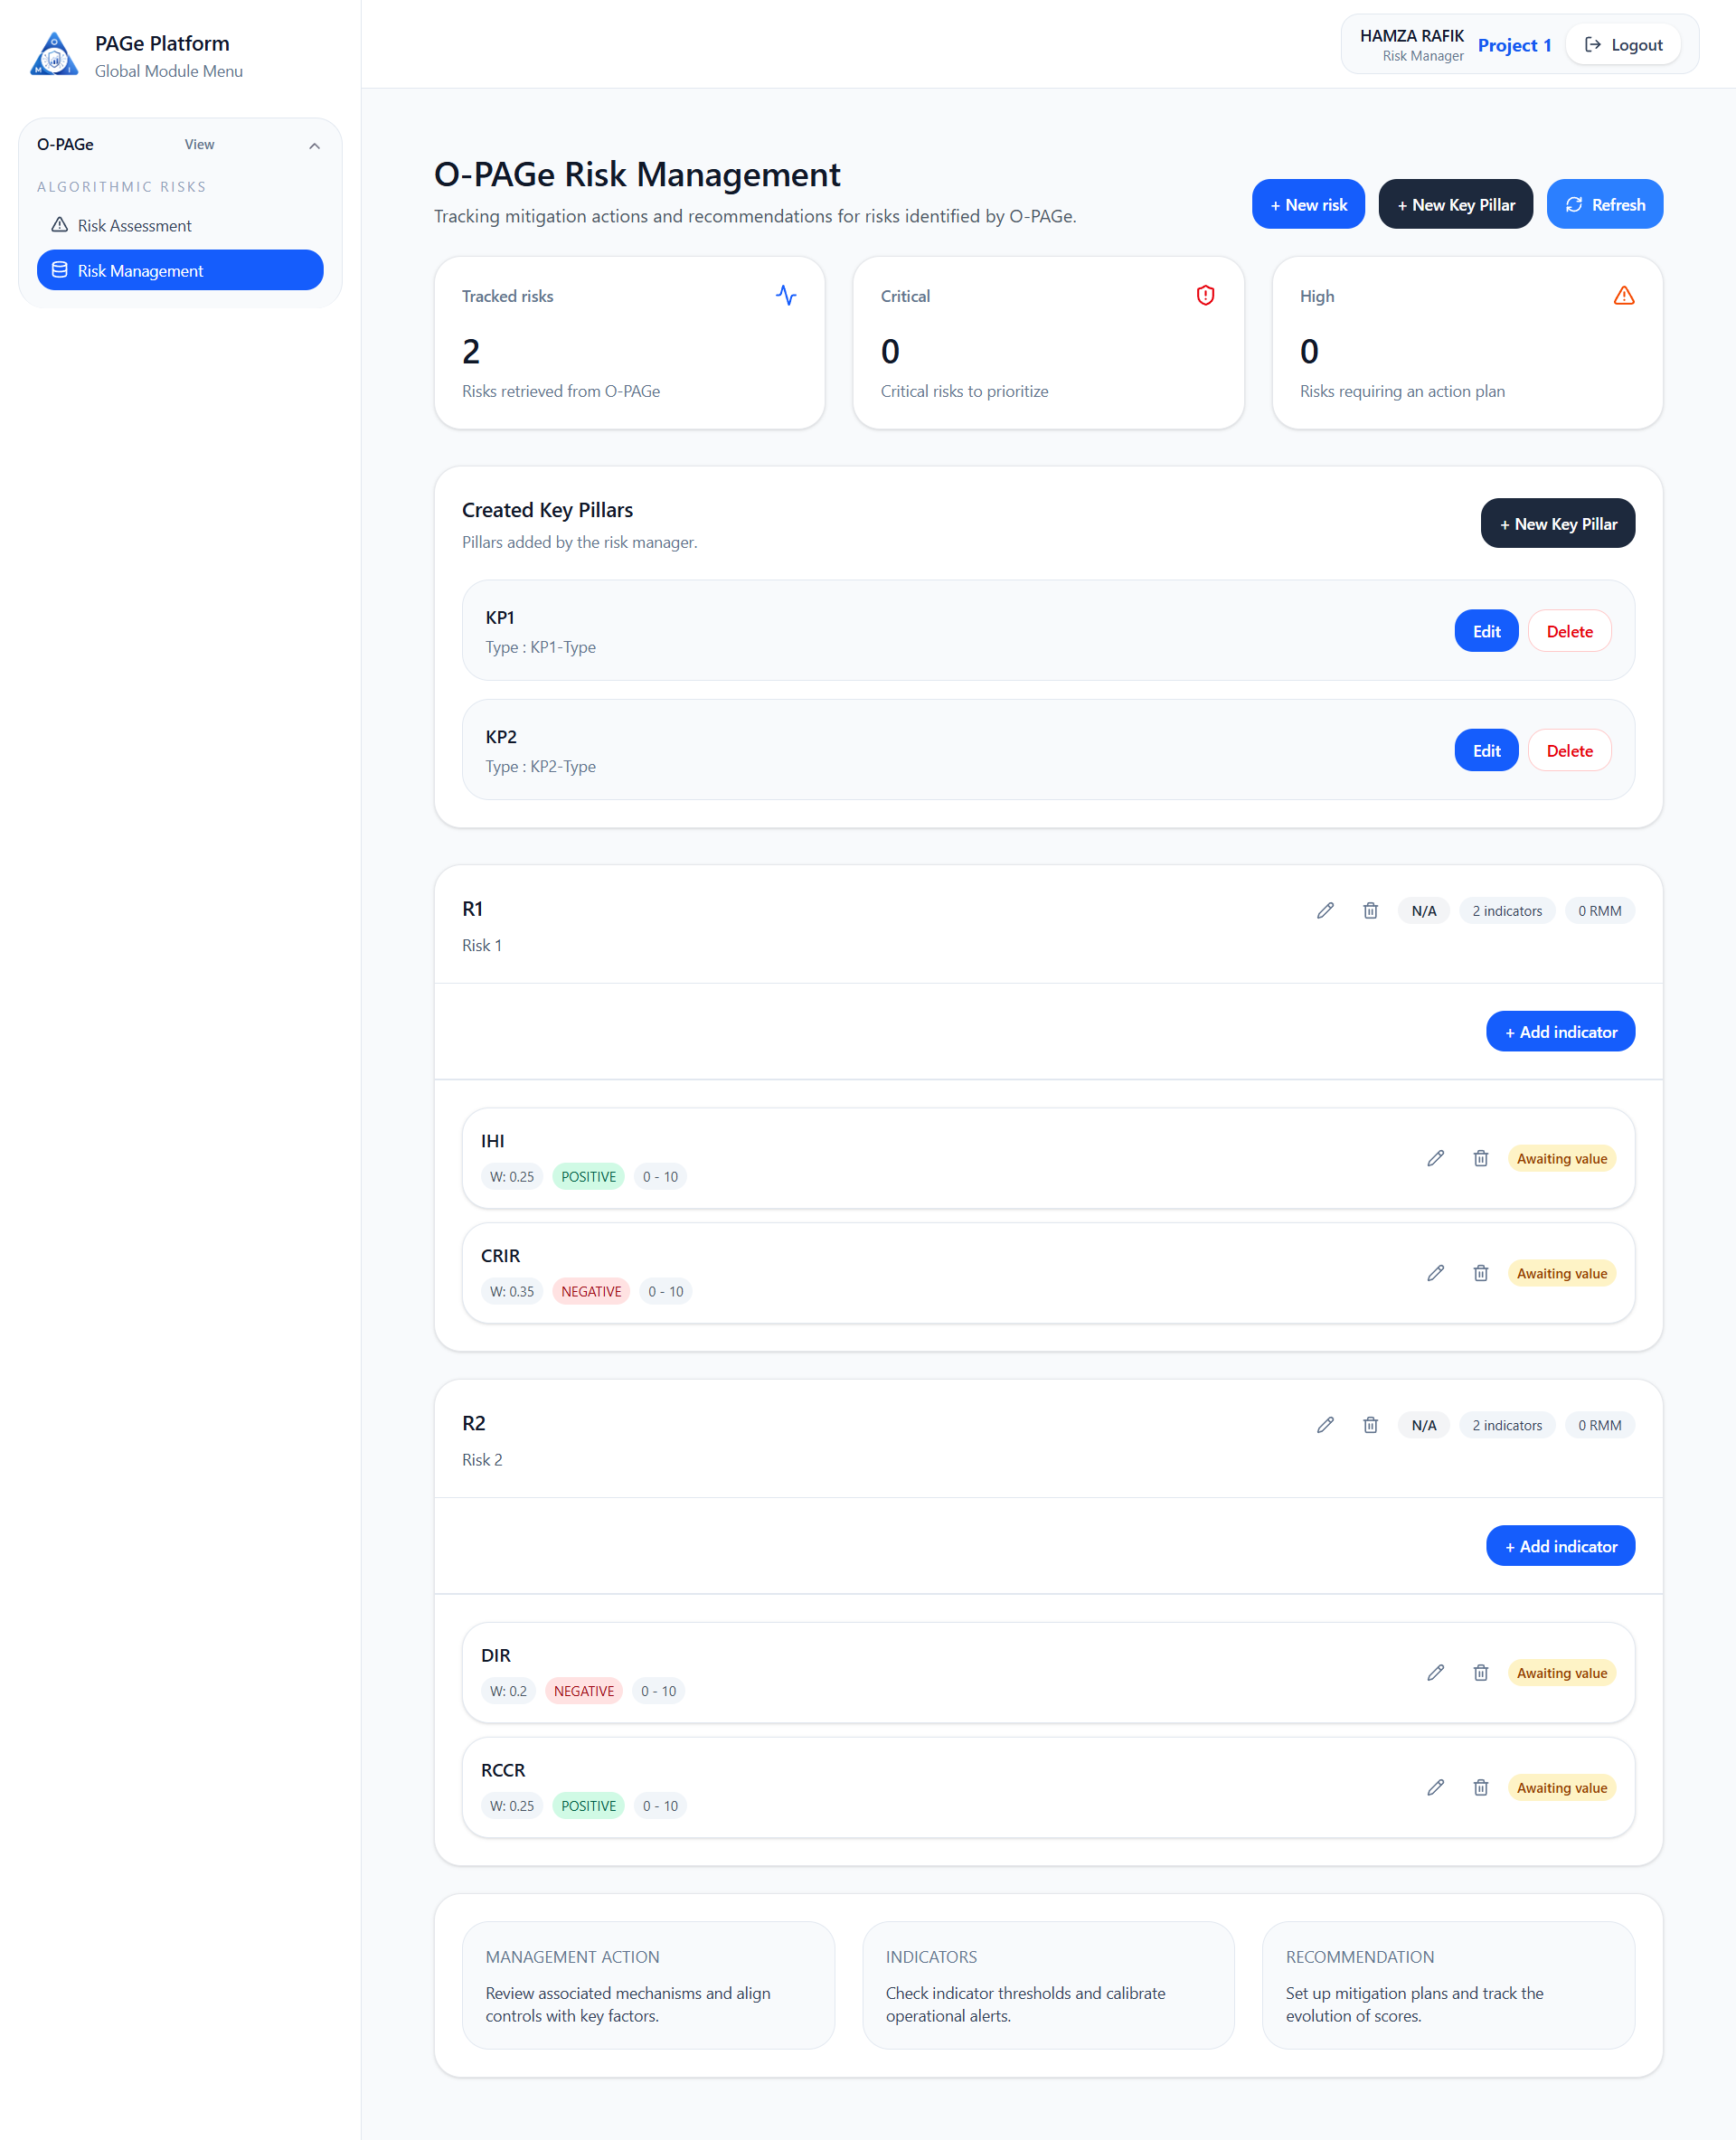
\includegraphics[width=0.8\textwidth]{Interfaces/Risk Manager/O-Page Risk Managment.png}
    \caption{Interface de gestion des risques}
\end{figure}
L'interface O-PAGe Risk Management est l'espace de travail réservé au Responsable des risques pour piloter la politique de gouvernance. Elle affiche des cartes de score analytiques mettant en évidence le nombre de menaces suivies et leur niveau de criticité. Ce tableau de bord permet d’ajouter et de structurer des Key Pillars, et de définir précisément des risques opérationnels avec leurs indicateurs.
\subsubsection{Consultation des risques}
\begin{figure}[H]
    \centering
    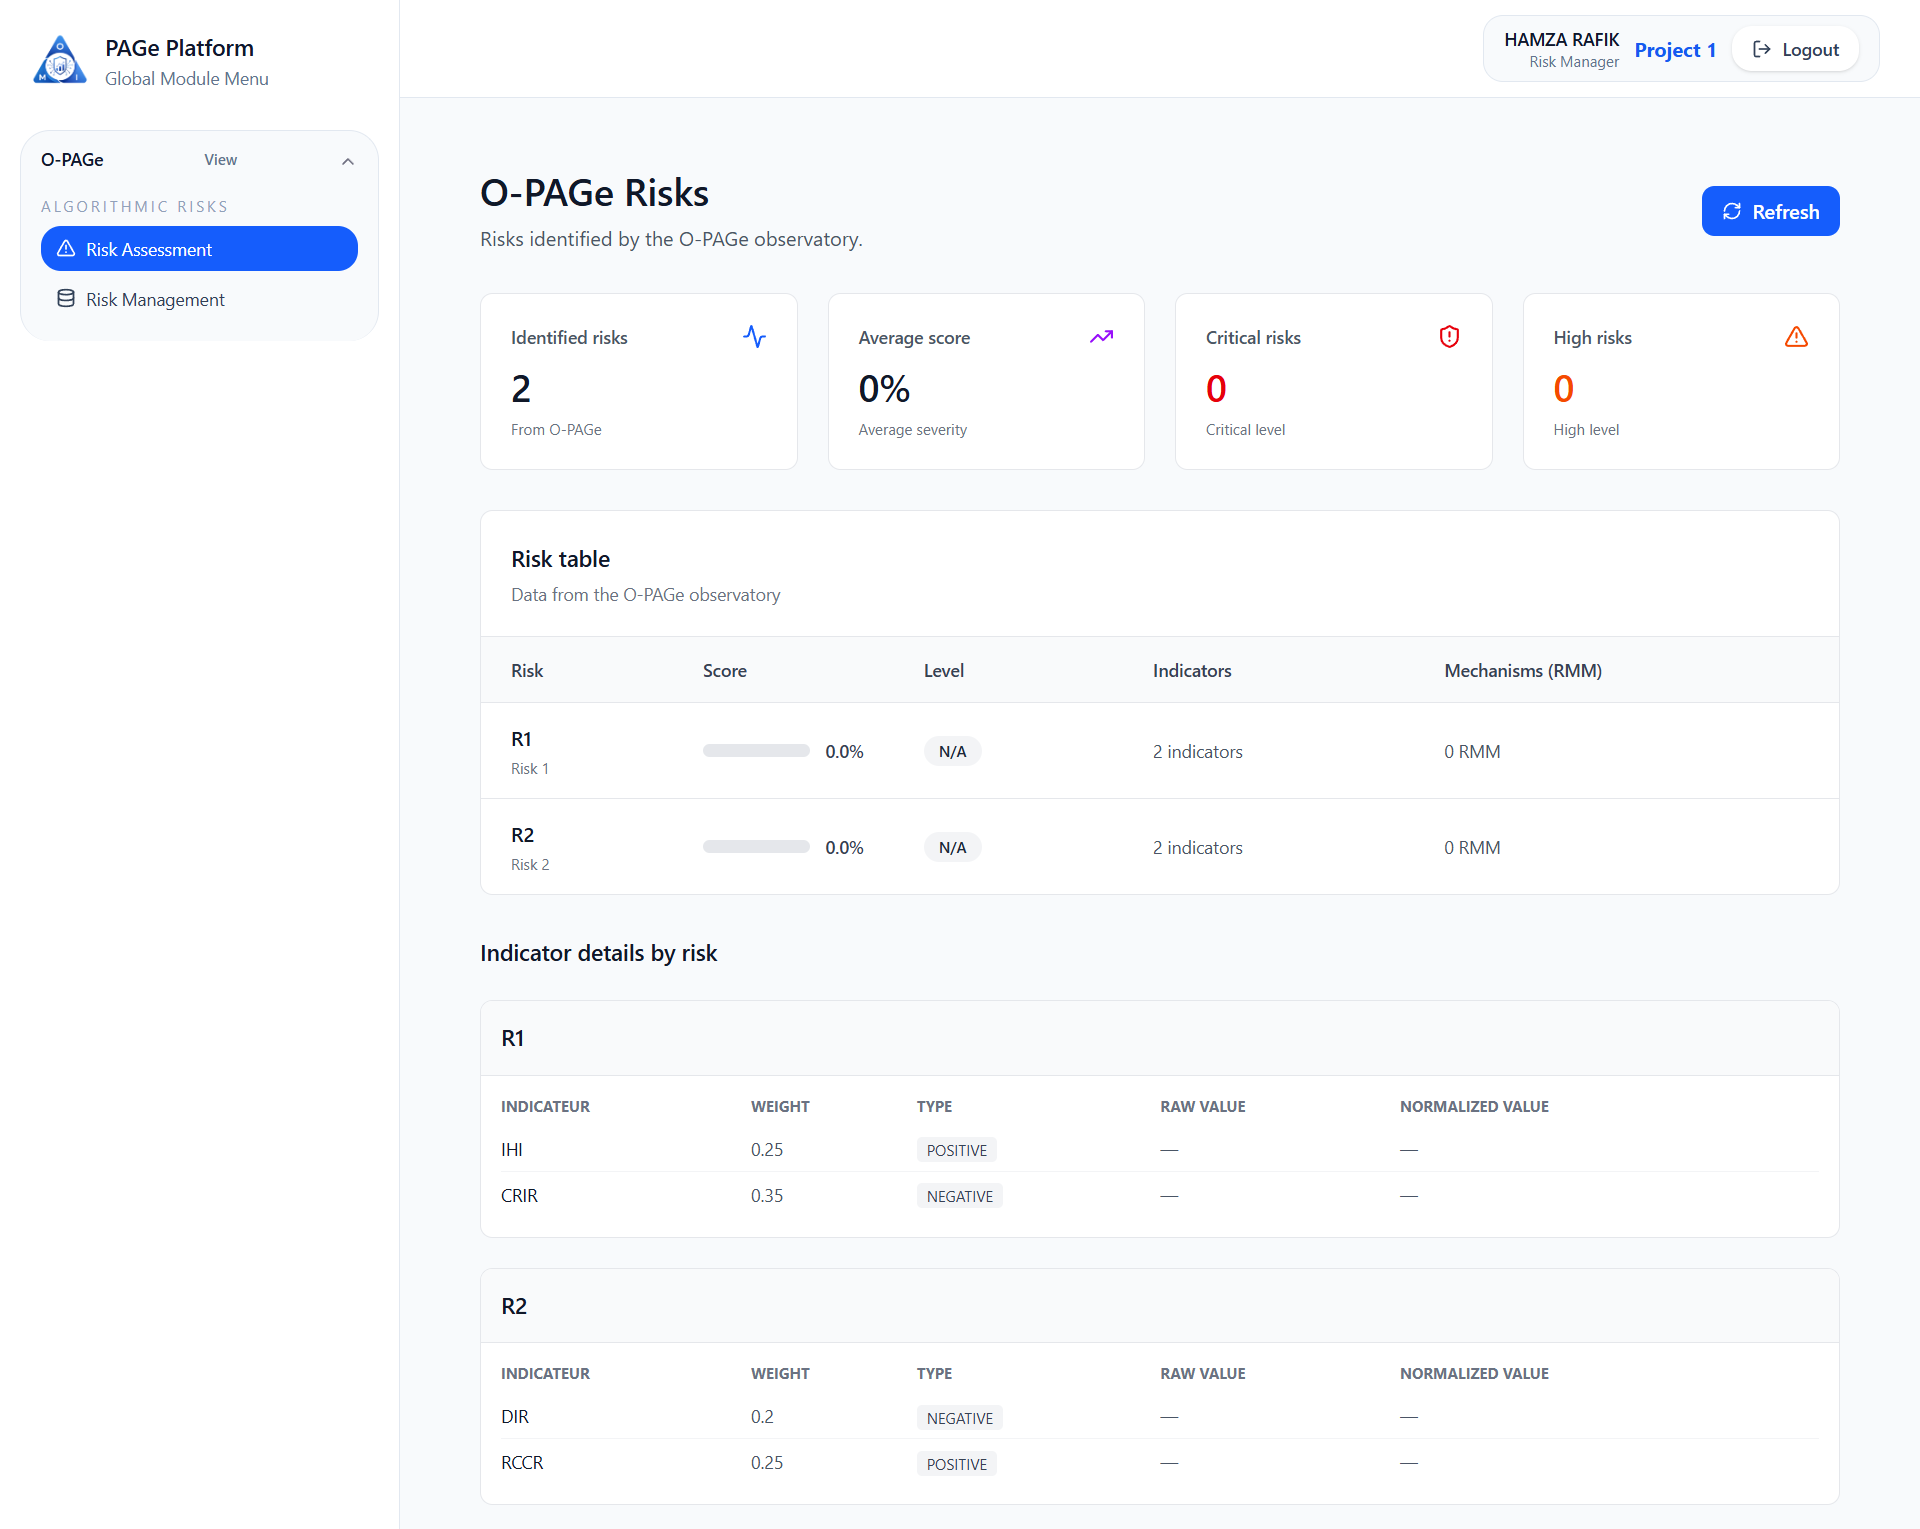
\includegraphics[width=0.8\textwidth]{Interfaces/Risk Manager/O-Page Risks.png}
    \caption{Interface de consultation des risques }
\end{figure}
L'interface O-PAGe Risks offre au Responsable des risques une vue d’ensemble analytique et consolidée des menaces identifiées. Elle présente des indicateurs de haut niveau tels que le score moyen de sévérité ou le nombre de risques critiques, complétés par un tableau de synthèse recensant les indicateurs rattachés et les mécanismes d'atténuation (RMM).
\subsection{Les interfaces de l'Organisateur Administratif}
\subsubsection{Le tableau de bord}
\begin{figure}[H]
    \centering
    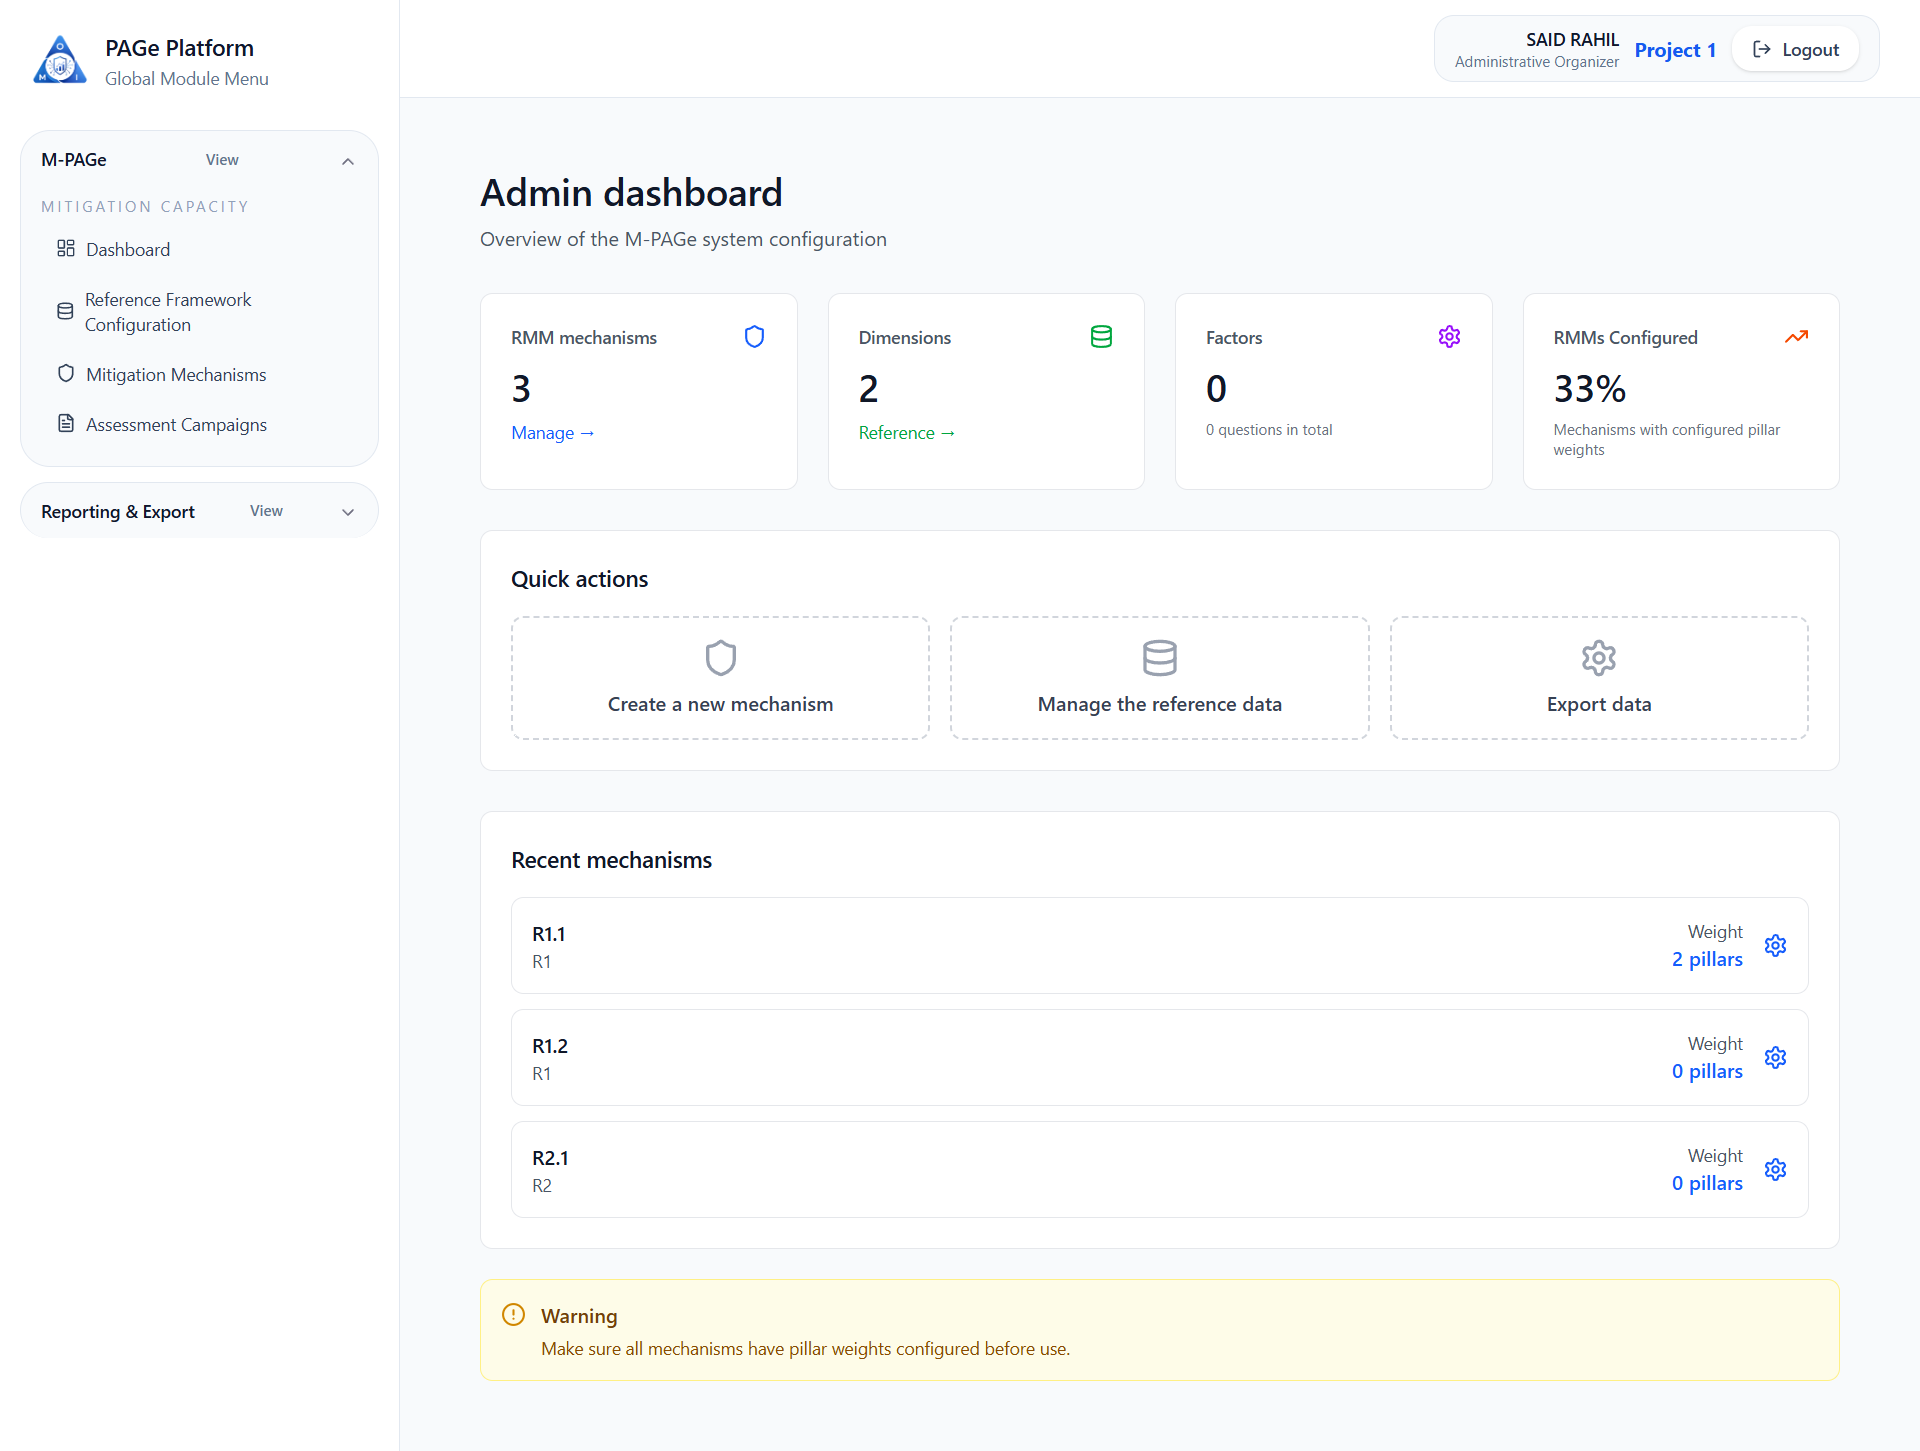
\includegraphics[width=0.8\textwidth]{Interfaces/Admin Organizer/Admin Dashboard.png}
    \caption{tableau de bord de l'organisateur administratif }
\end{figure}
L'interface Admin dashboard offre une vue globale et synthétique sur la configuration du système. Ce tableau de bord affiche des cartes de performance clés qui quantifient les mécanismes RMM, les dimensions et le taux de mécanismes configurés. L’interface intègre également une section d'actions rapides pour créer un mécanisme ou exporter des données, ainsi qu'une liste dynamique des mécanismes récents permettant de vérifier instantanément leur état de pondération.
\subsubsection{Configuration des référentiels}
\begin{figure}[H]
    \centering
    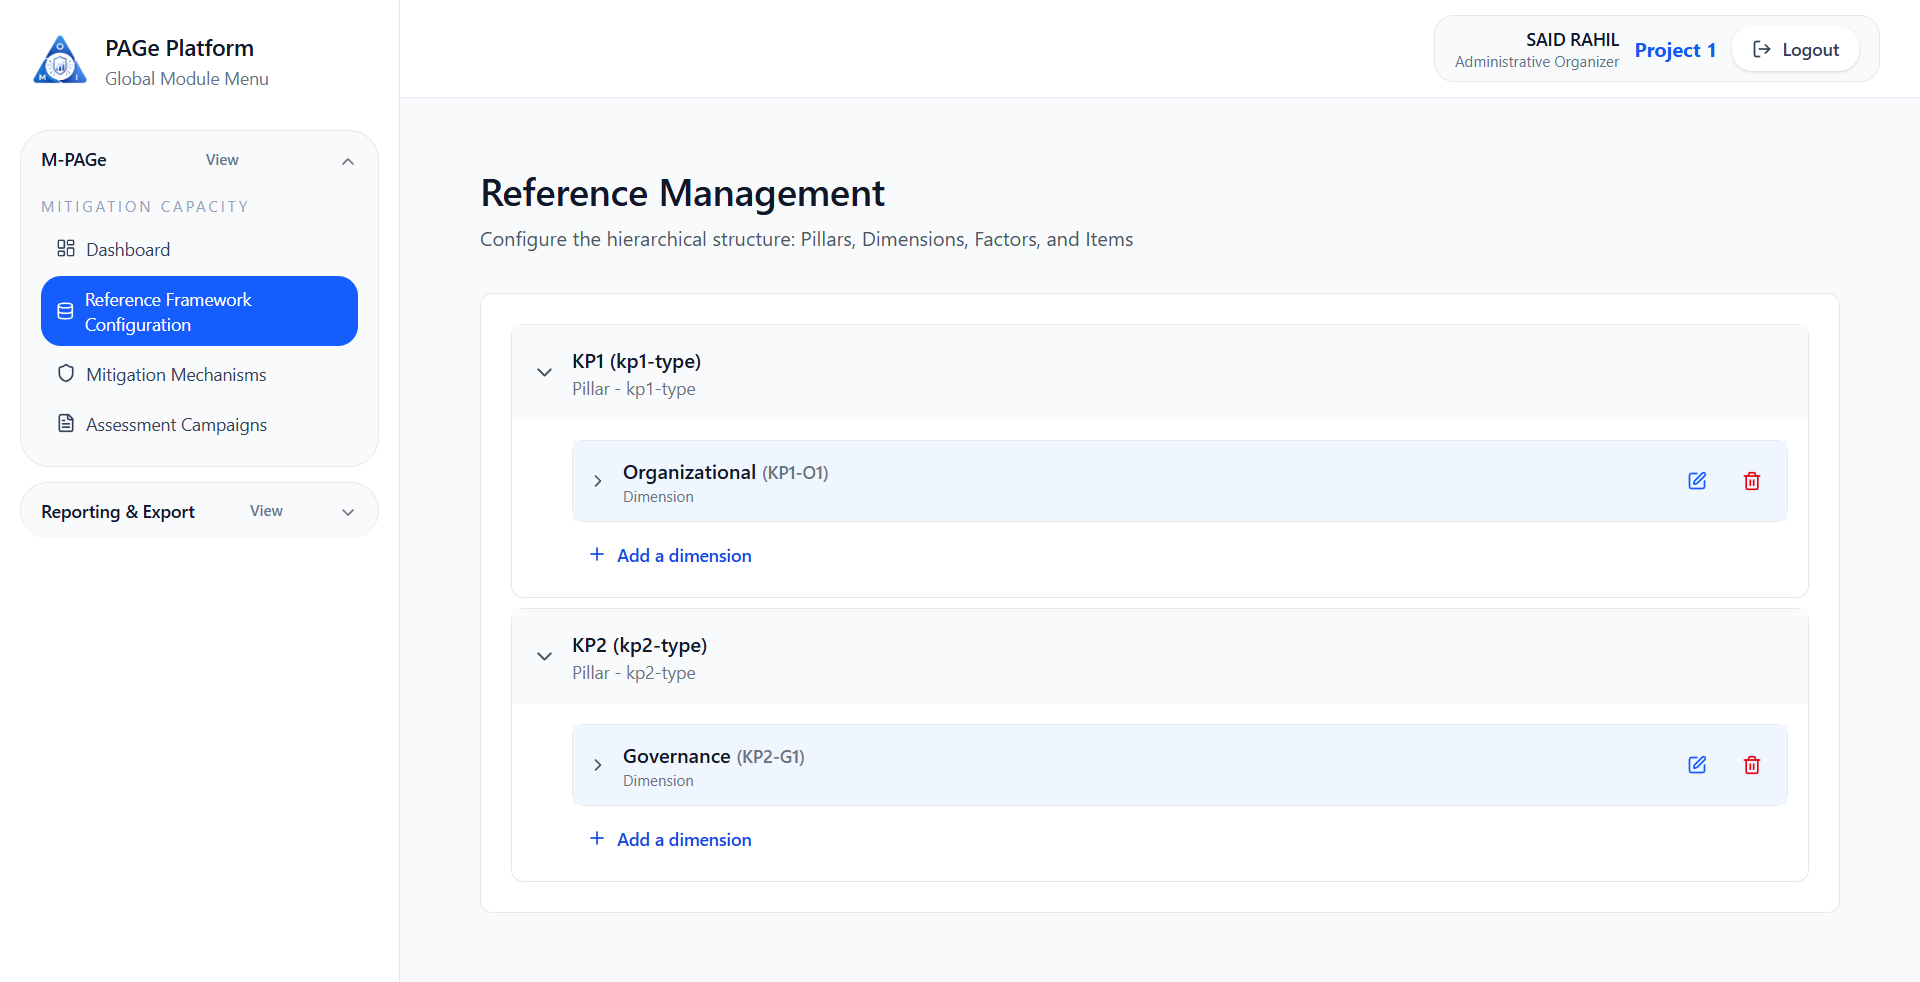
\includegraphics[width=0.8\textwidth]{Interfaces/Admin Organizer/Reference Management (Add Dimensions).png}
    \caption{Interface de gestion des dimensions}
\end{figure}
L'interface Reference Management permet à l'Organisateur Administratif de gérer la structure du projet. Depuis cet espace, l'utilisateur peut consulter la liste des piliers clés (Key Pillars) enregistrés dans le système. De plus, elle offre la possibilité d'ajouter de nouvelles dimensions à chaque pilier à l'aide d'un bouton dédié, afin de compléter pas à pas le référentiel.
\subsubsection{Configuration des mécanismes}
\begin{figure}[H]
    \centering
    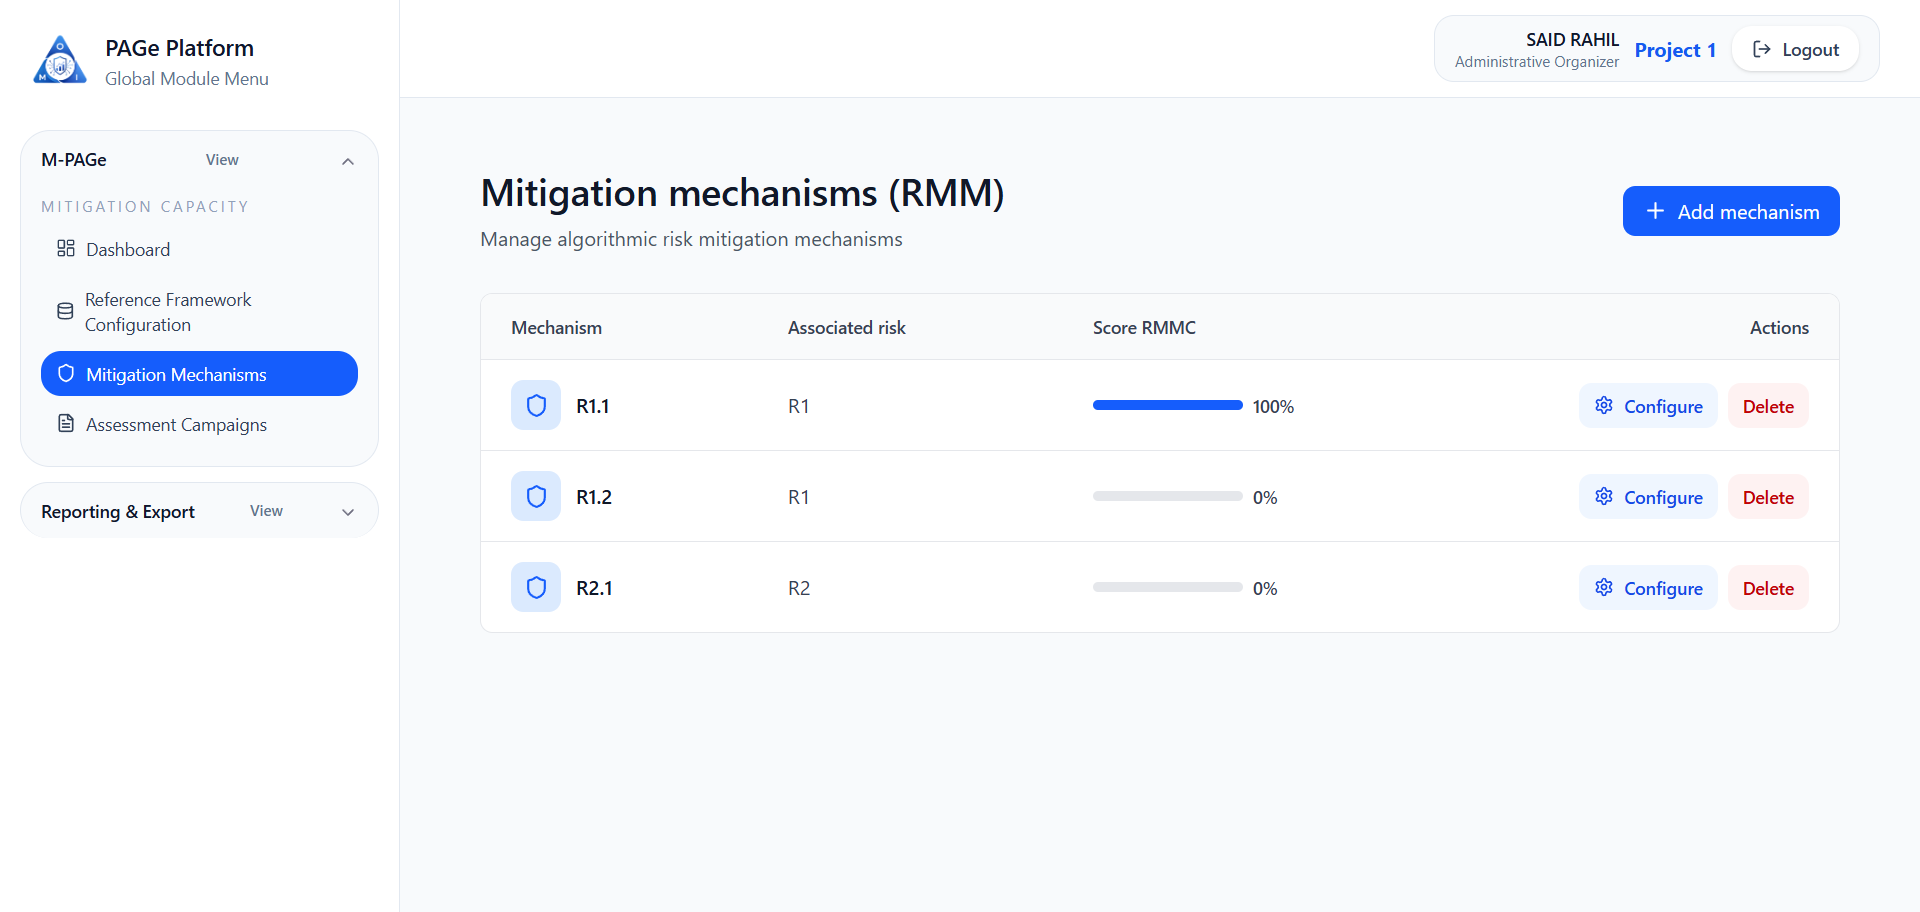
\includegraphics[width=0.8\textwidth]{Interfaces/Admin Organizer/Mitigation mechanisms (RMM).png}
    \caption{Interface de gestion des mécanismes}
\end{figure}
Cet espace affiche un tableau regroupant les différents mécanismes, les risques associés et leur score RMMC. À l'aide de boutons d'action dédiés, l'utilisateur peut supprimer un élément existant ou choisir de le configurer en attribuant un poids spécifique à chaque Key Pillar.
\subsubsection{Lancement des campagnes d'évaluation}
\begin{figure}[H]
    \centering
    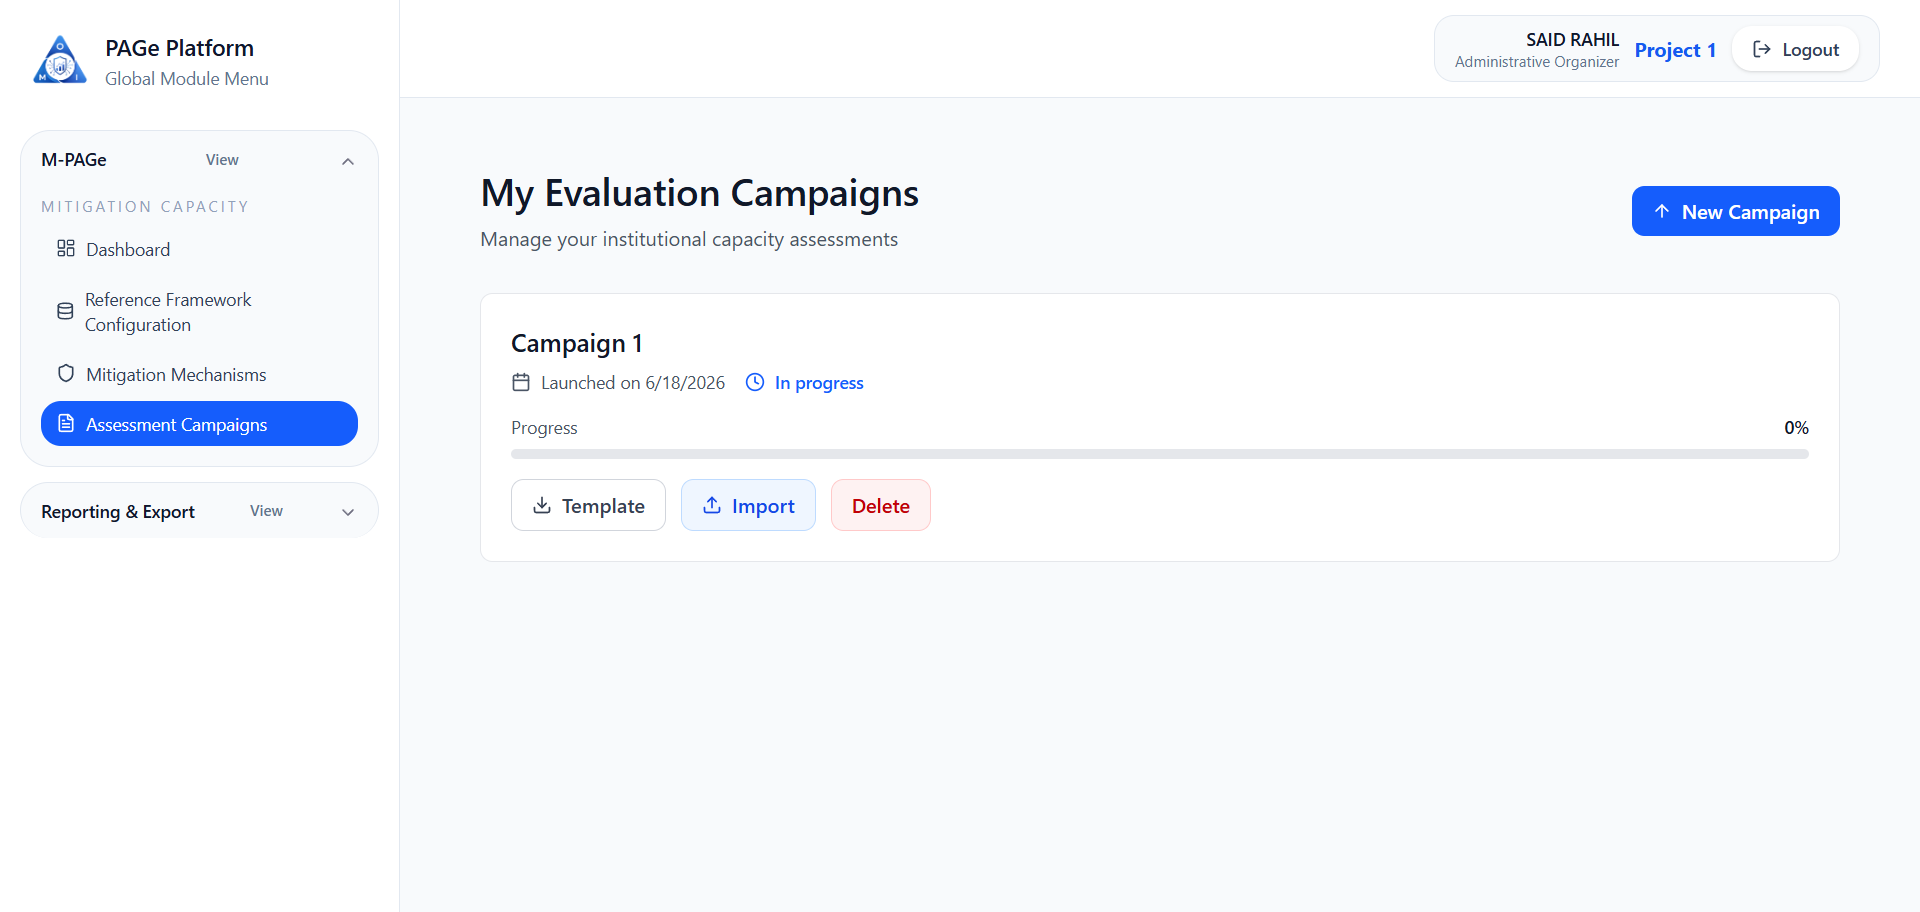
\includegraphics[width=0.8\textwidth]{Interfaces/Admin Organizer/Evaluation Campaigns.png}
    \caption{Interface de gestion des campagnes }
\end{figure}
L'interface My Evaluation Campaigns permet à l'Organisateur Administratif de piloter les évaluations de la plateforme. Grâce au bouton New Campaign , l'utilisateur peut lancer une nouvelle campagne d'évaluation pour le projet en cours. Cet espace affiche également la liste des campagnes actives avec leur date de lancement et leur progression en temps réel, tout en offrant la possibilité de supprimer une campagne existante via le bouton Delete.
\subsection{Les interfaces de l'Observateur}
\subsubsection{Tableau de bord}
\begin{figure}[H]
    \centering
    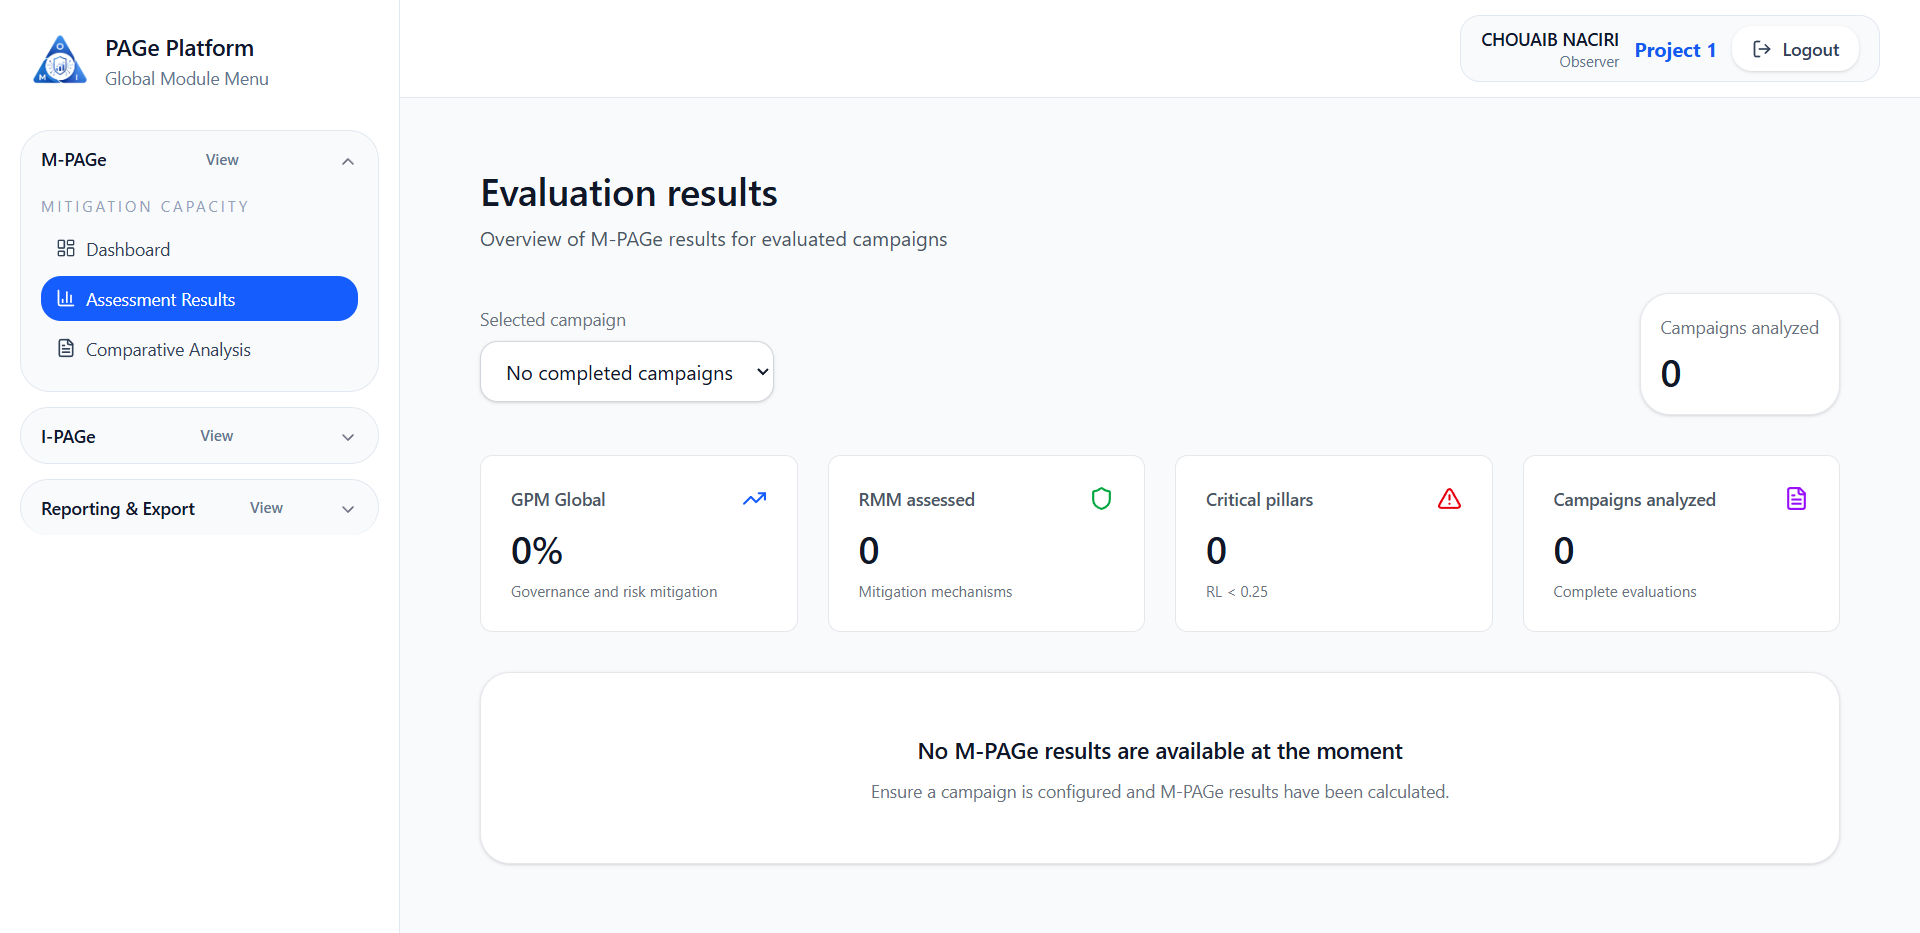
\includegraphics[width=0.8\textwidth]{Interfaces/Observer/Observer Dashboard.png}
    \caption{Tableau de bord de l'observateur }
\end{figure}
L'interface Evaluation results constitue le tableau de bord principal de l'Observateur pour le suivi des campagnes finalisées. Cet espace permet à l'utilisateur de sélectionner une campagne spécifique afin de consulter ses résultats globaux. L'interface affiche des indicateurs clés concernant le score global de gouvernance (GPM Global), les mécanismes atténués (RMM assessed), les piliers critiques et le nombre total d'évaluations analysées pour le projet
\subsubsection{Comparaison avant/après mitigation}
\begin{figure}[H]
    \centering
    
\includegraphics[width=0.8\textwidth]{Interfaces/Observer/Comparative analysis.png}
    \caption{Interface de comparaison}
\end{figure}
L'interface Comparative analysis  permet à l'Observateur de confronter les données de la plateforme. Cet espace offre la possibilité de sélectionner deux évaluations distinctes afin de comparer directement leurs résultats côte à côte. Cet outil permet ainsi de mesurer l'évolution de la situation et d'évaluer l'impact des actions menées avant et après la mise en place de la mitigation.
\subsection{Les interfaces de Responsable Organisationnel}
\subsubsection{Tableau de bord}
\begin{figure}[H]
    \centering
    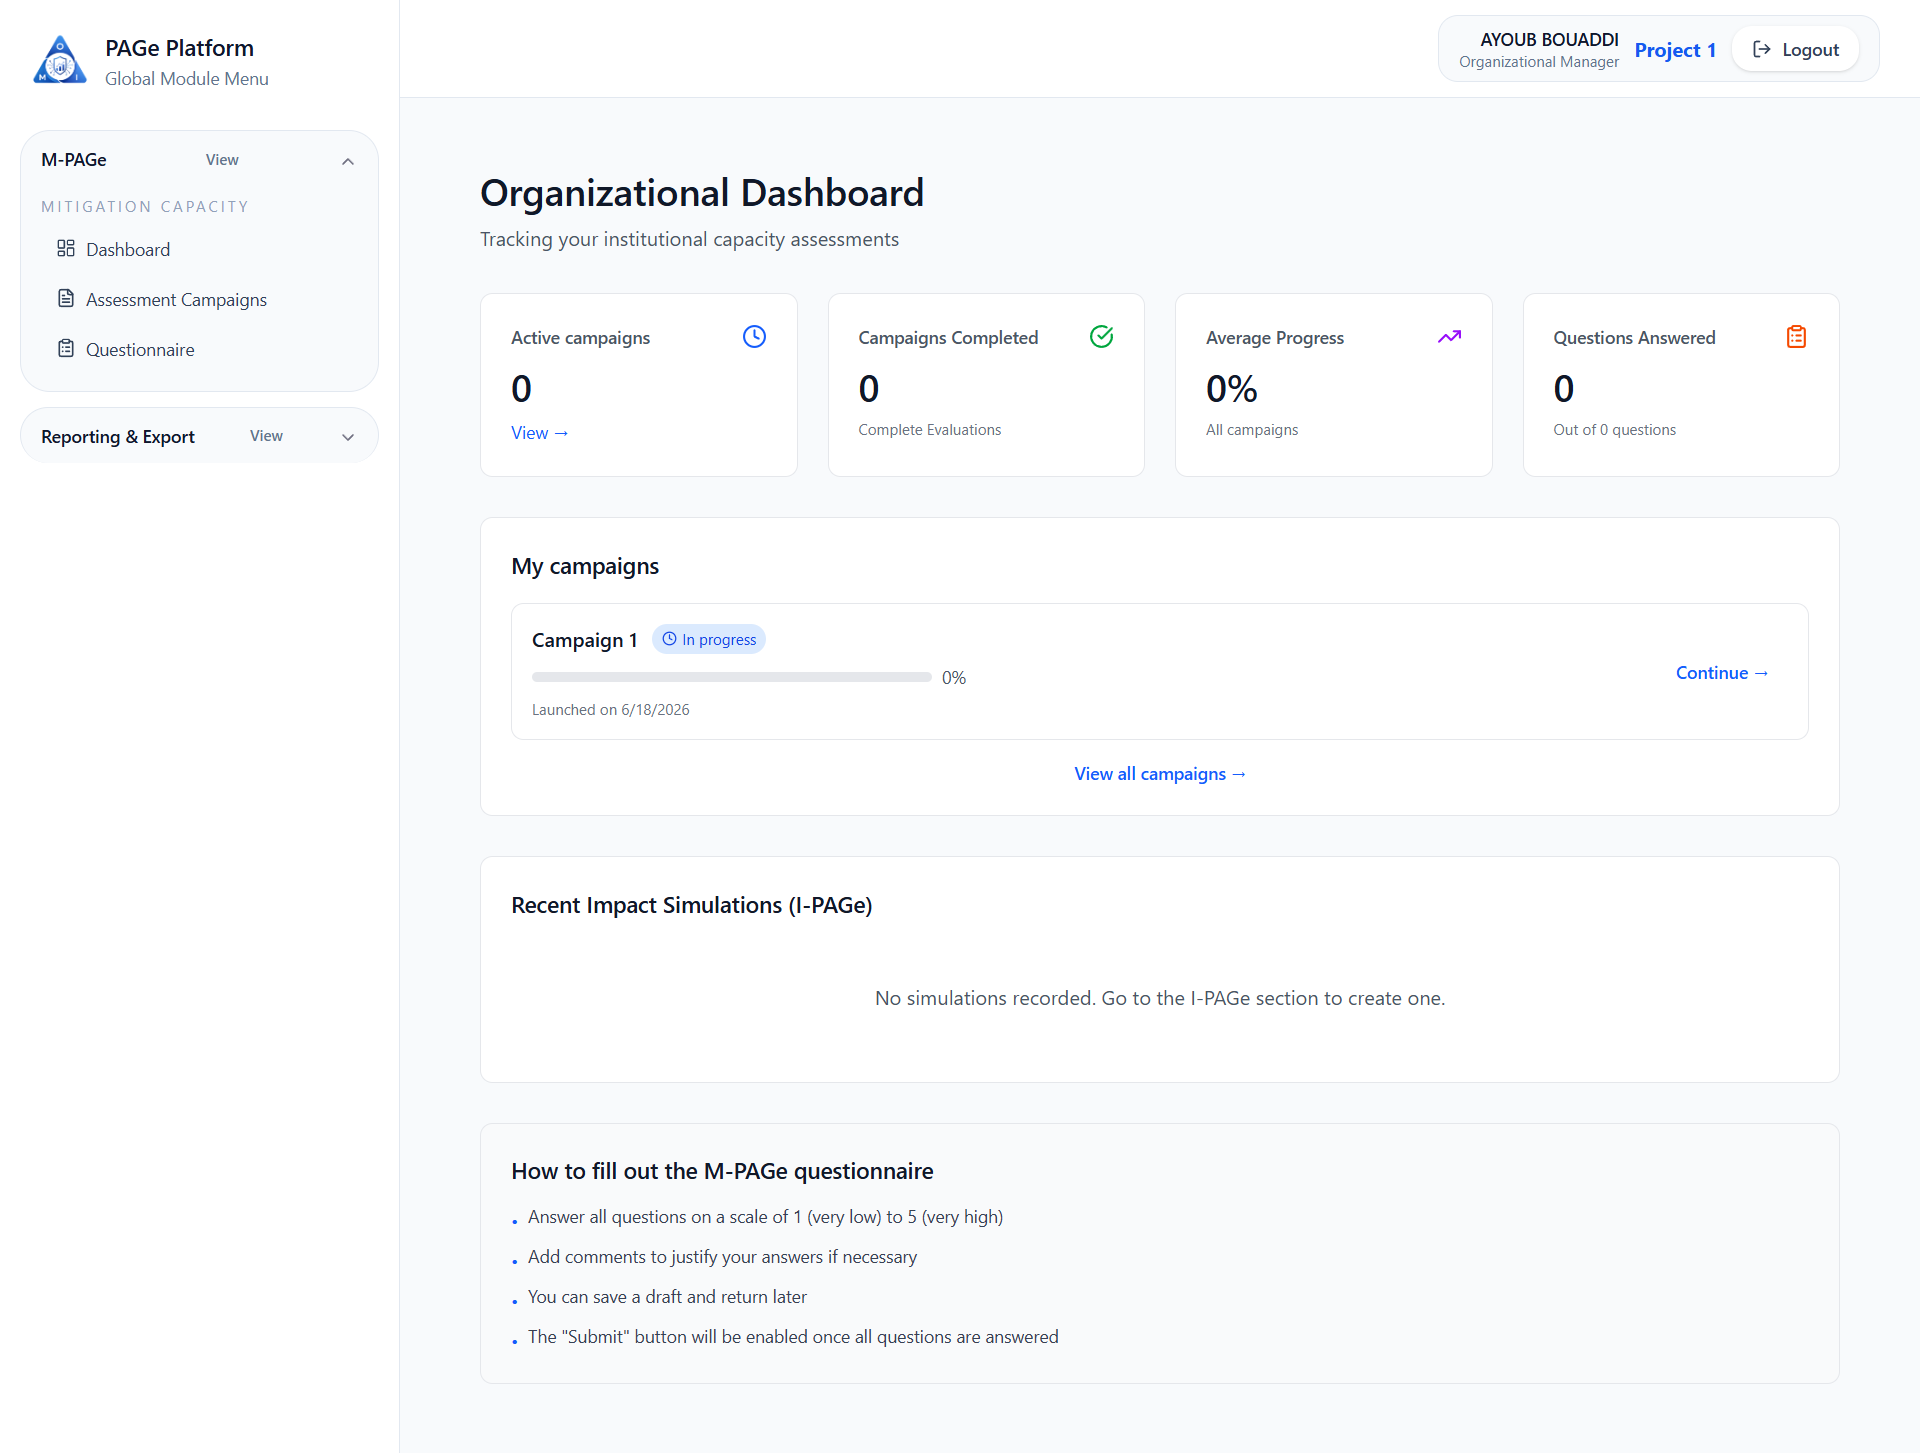
\includegraphics[width=0.7\textwidth]{Interfaces/Org Manager/Organizational Dashboard.png}
    \caption{Tableau de bord de Responsable organisationnel }
\end{figure}
L'interface Organizational Dashboard est le tableau de bord principal du Responsable Organisationnel pour le suivi des évaluations de capacité institutionnelle. Elle affiche des indicateurs clés comme le nombre de campagnes actives, complétées, la progression moyenne et le total des questions répondues. Cet espace liste également les campagnes en cours pour permettre à l'utilisateur de poursuivre le remplissage de ses questionnaires, tout en intégrant un bloc récapitulatif des simulations d'impact récentes.
\subsubsection{Suivi de l'avancement des campagnes}
\begin{figure}[H]
    \centering
    
\includegraphics[width=0.8\textwidth]{Interfaces/Org Manager/Evaluation Campaigns.png}
    \caption{Interface de suivi des campagnes}
\end{figure}
L'interface My Evaluation Campaigns permet au responsable organisationnel de piloter les évaluations de la plateforme. Grâce au bouton New Campaign , l'utilisateur peut lancer une nouvelle campagne d'évaluation pour le projet en cours. Cet espace affiche également la liste des campagnes actives avec leur date de lancement et leur progression en temps réel, tout en offrant la possibilité de supprimer une campagne existante via le bouton Delete.
\subsubsection{Saisie les réponses d'évaluation}
\begin{figure}[H]
    \centering
    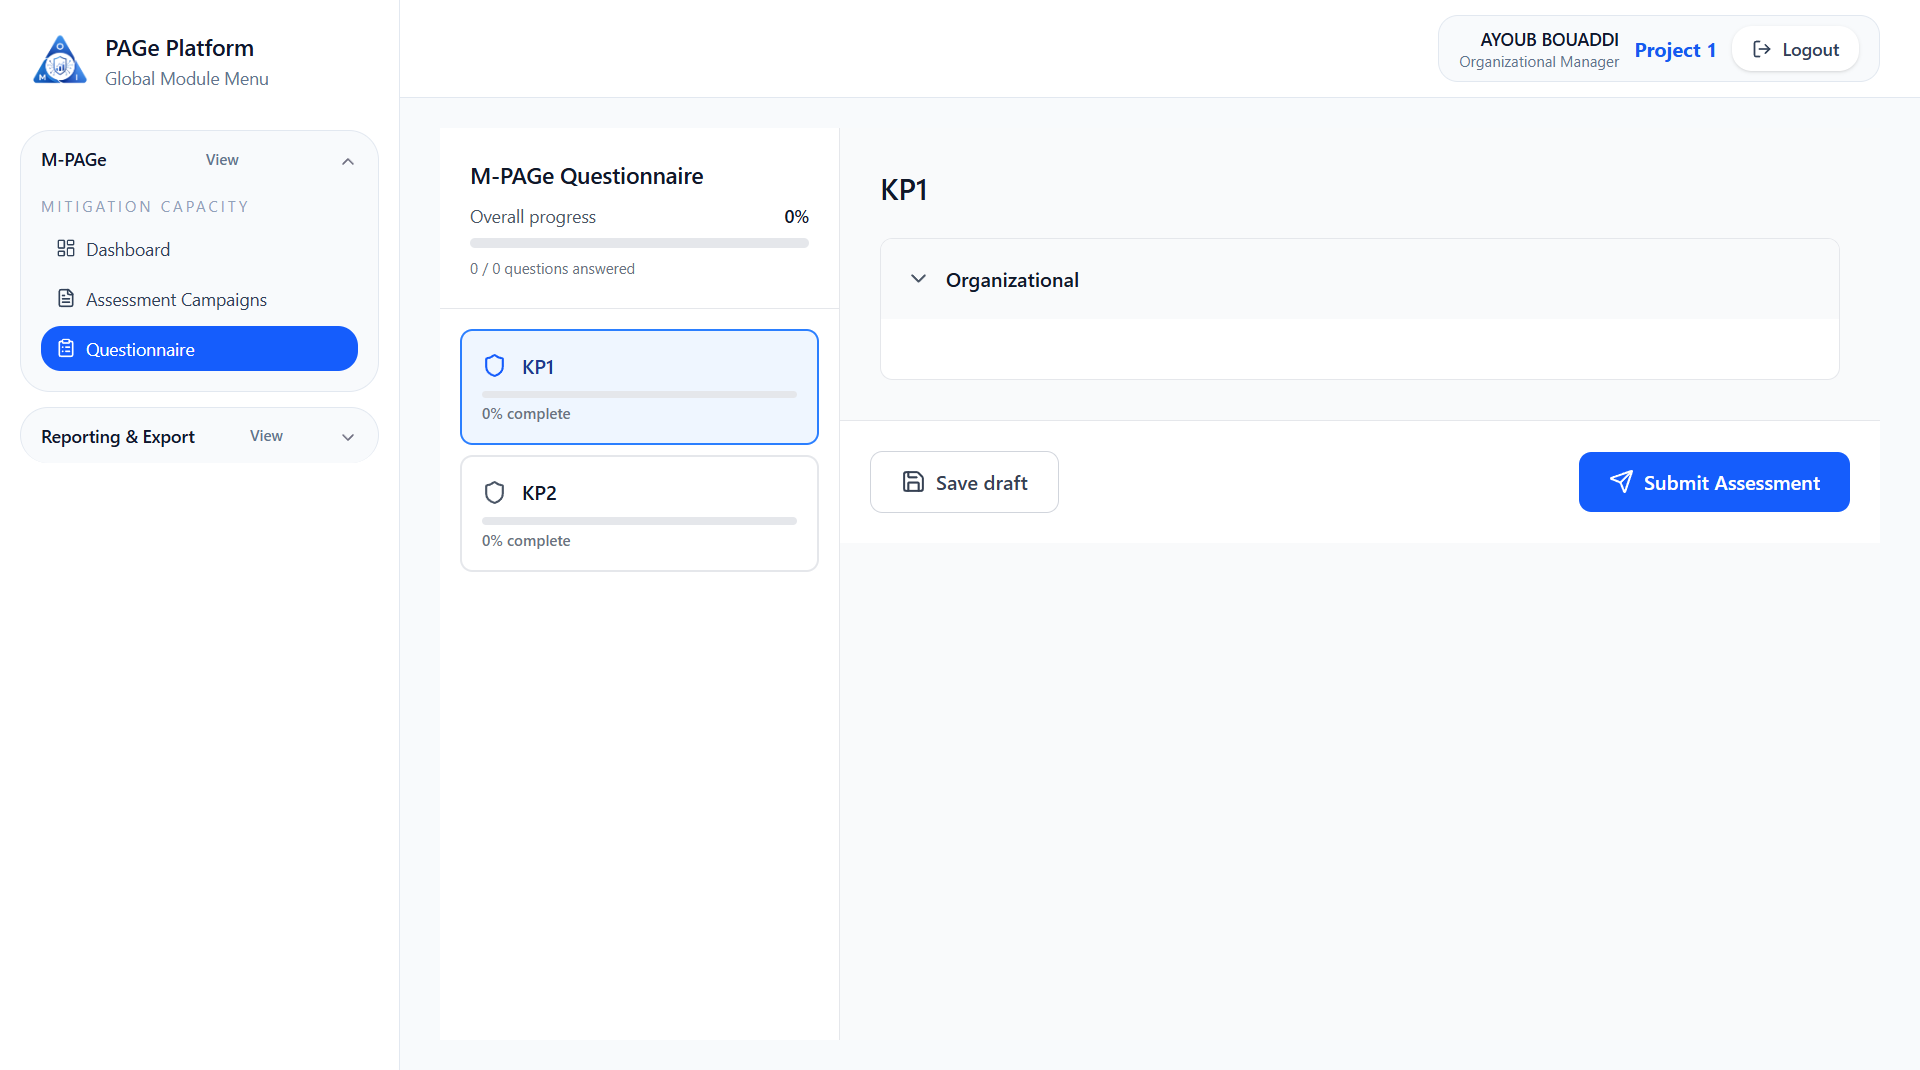
\includegraphics[width=0.8\textwidth]{Interfaces/Org Manager/M-PAGe Questionnaire.png}
    \caption{Interface de saisie les réponses d'évaluation }
\end{figure}
L'interface M-PAGe Questionnaire permet au Responsable Organisationnel de saisir les réponses aux campagnes d'évaluation. Cet espace est structuré par piliers clés, affichant un indicateur de progression en temps réel pour chacun d'eux ainsi que l'avancement global du formulaire. L'utilisateur peut y remplir les sections requises, sauvegarder ses saisies à tout moment grâce au bouton Save draft, puis valider définitivement sa contribution via le bouton Submit Assessment.
\subsubsection{Export les rapports}
\begin{figure}[H]
    \centering
    
\includegraphics[width=0.7\textwidth]{Interfaces/Org Manager/Export Data.png}
    \caption{Interface d'export les rapports }
\end{figure}
L'interface Export Data permet au Responsable Organisationnel de télécharger les synthèses de ses évaluations. Cet espace offre la possibilité de sélectionner un projet et une campagne spécifique afin de générer le rapport correspondant. À l'aide de boutons d'action épurés, l'utilisateur peut choisir d'exporter ses données et graphiques directement au format CSV ou au format PDF selon ses besoins.
\subsection{Les interfaces de Décideur}
\subsubsection{Configuration les paramètres de simulation}
\begin{figure}[H]
    \centering
    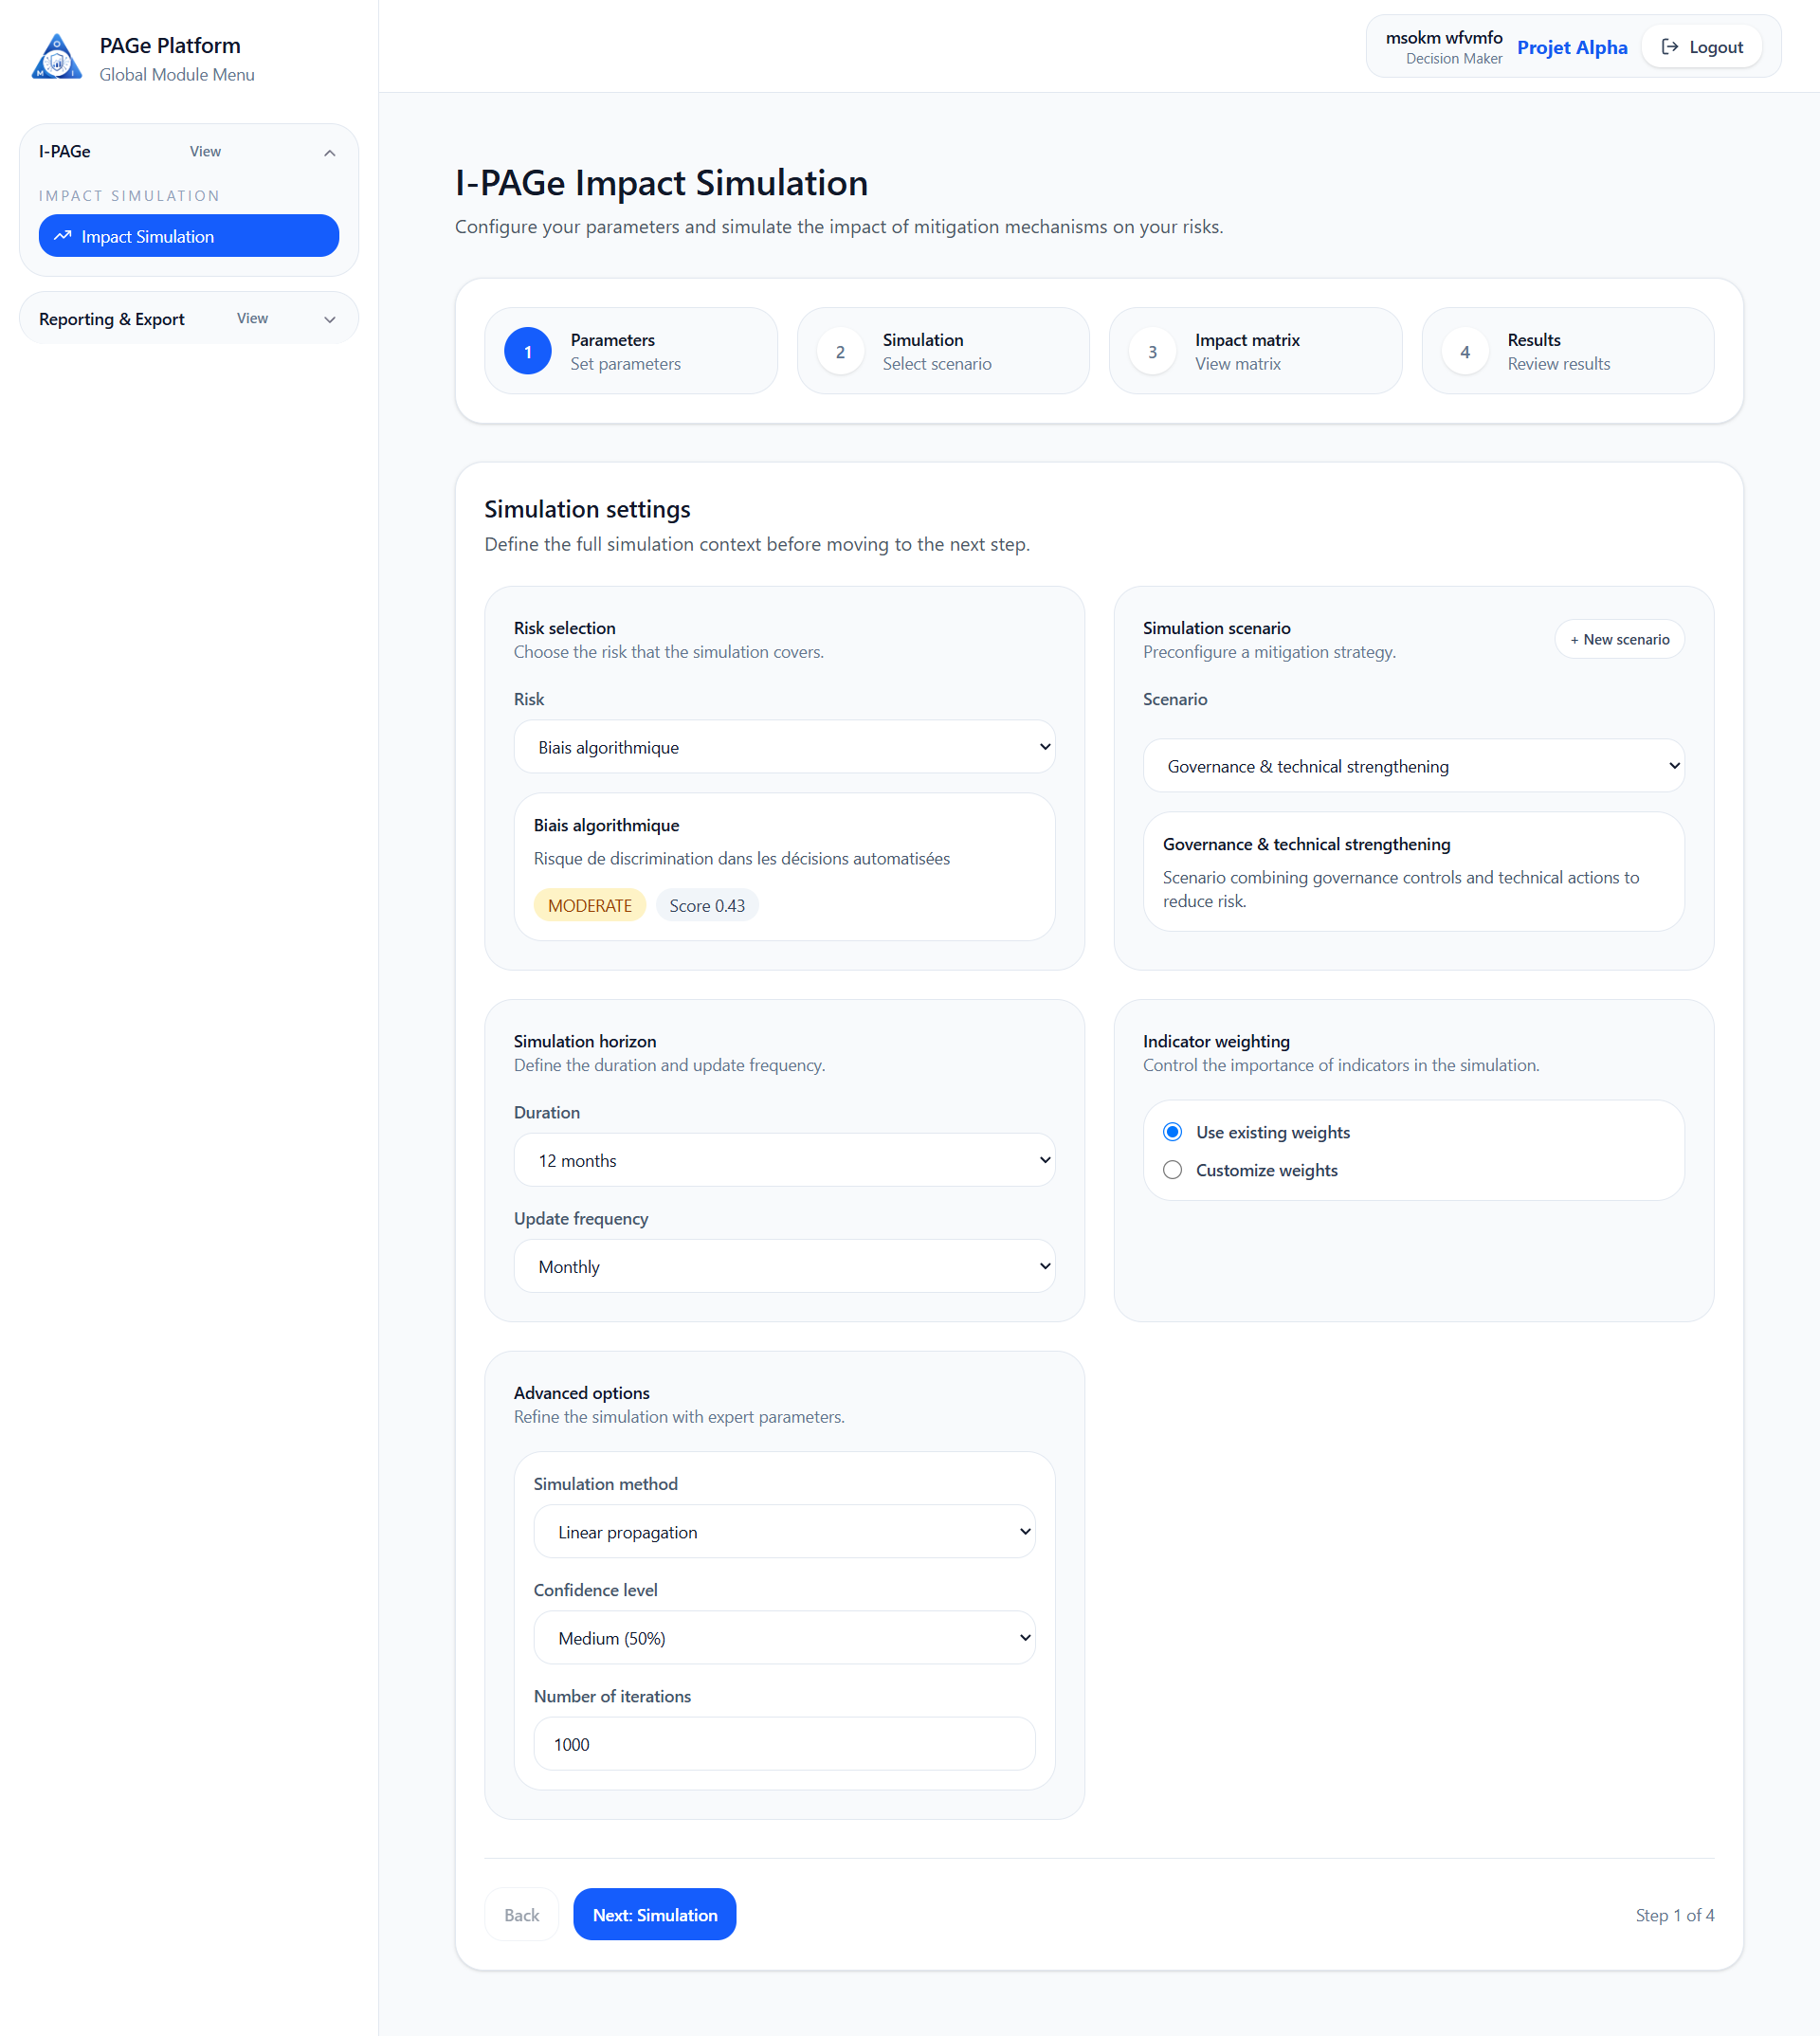
\includegraphics[width=0.8\textwidth]{Interfaces/Decision Maker/Impact Simulation.png}
    \caption{Interface des paramètres}
\end{figure}
L'interface I-PAGe Impact Simulation permet au Décideur de paramétrer les simulations pour évaluer l'effet des mécanismes d'atténuation sur les risques. Cet espace propose un parcours guidé en quatre étapes, à commencer par la définition du contexte via l'onglet Simulation settings. L'utilisateur peut y sélectionner un risque, choisir un scénario, déterminer l'horizon temporel ainsi que la pondération des indicateurs.

\begin{figure}[H]
    \centering
    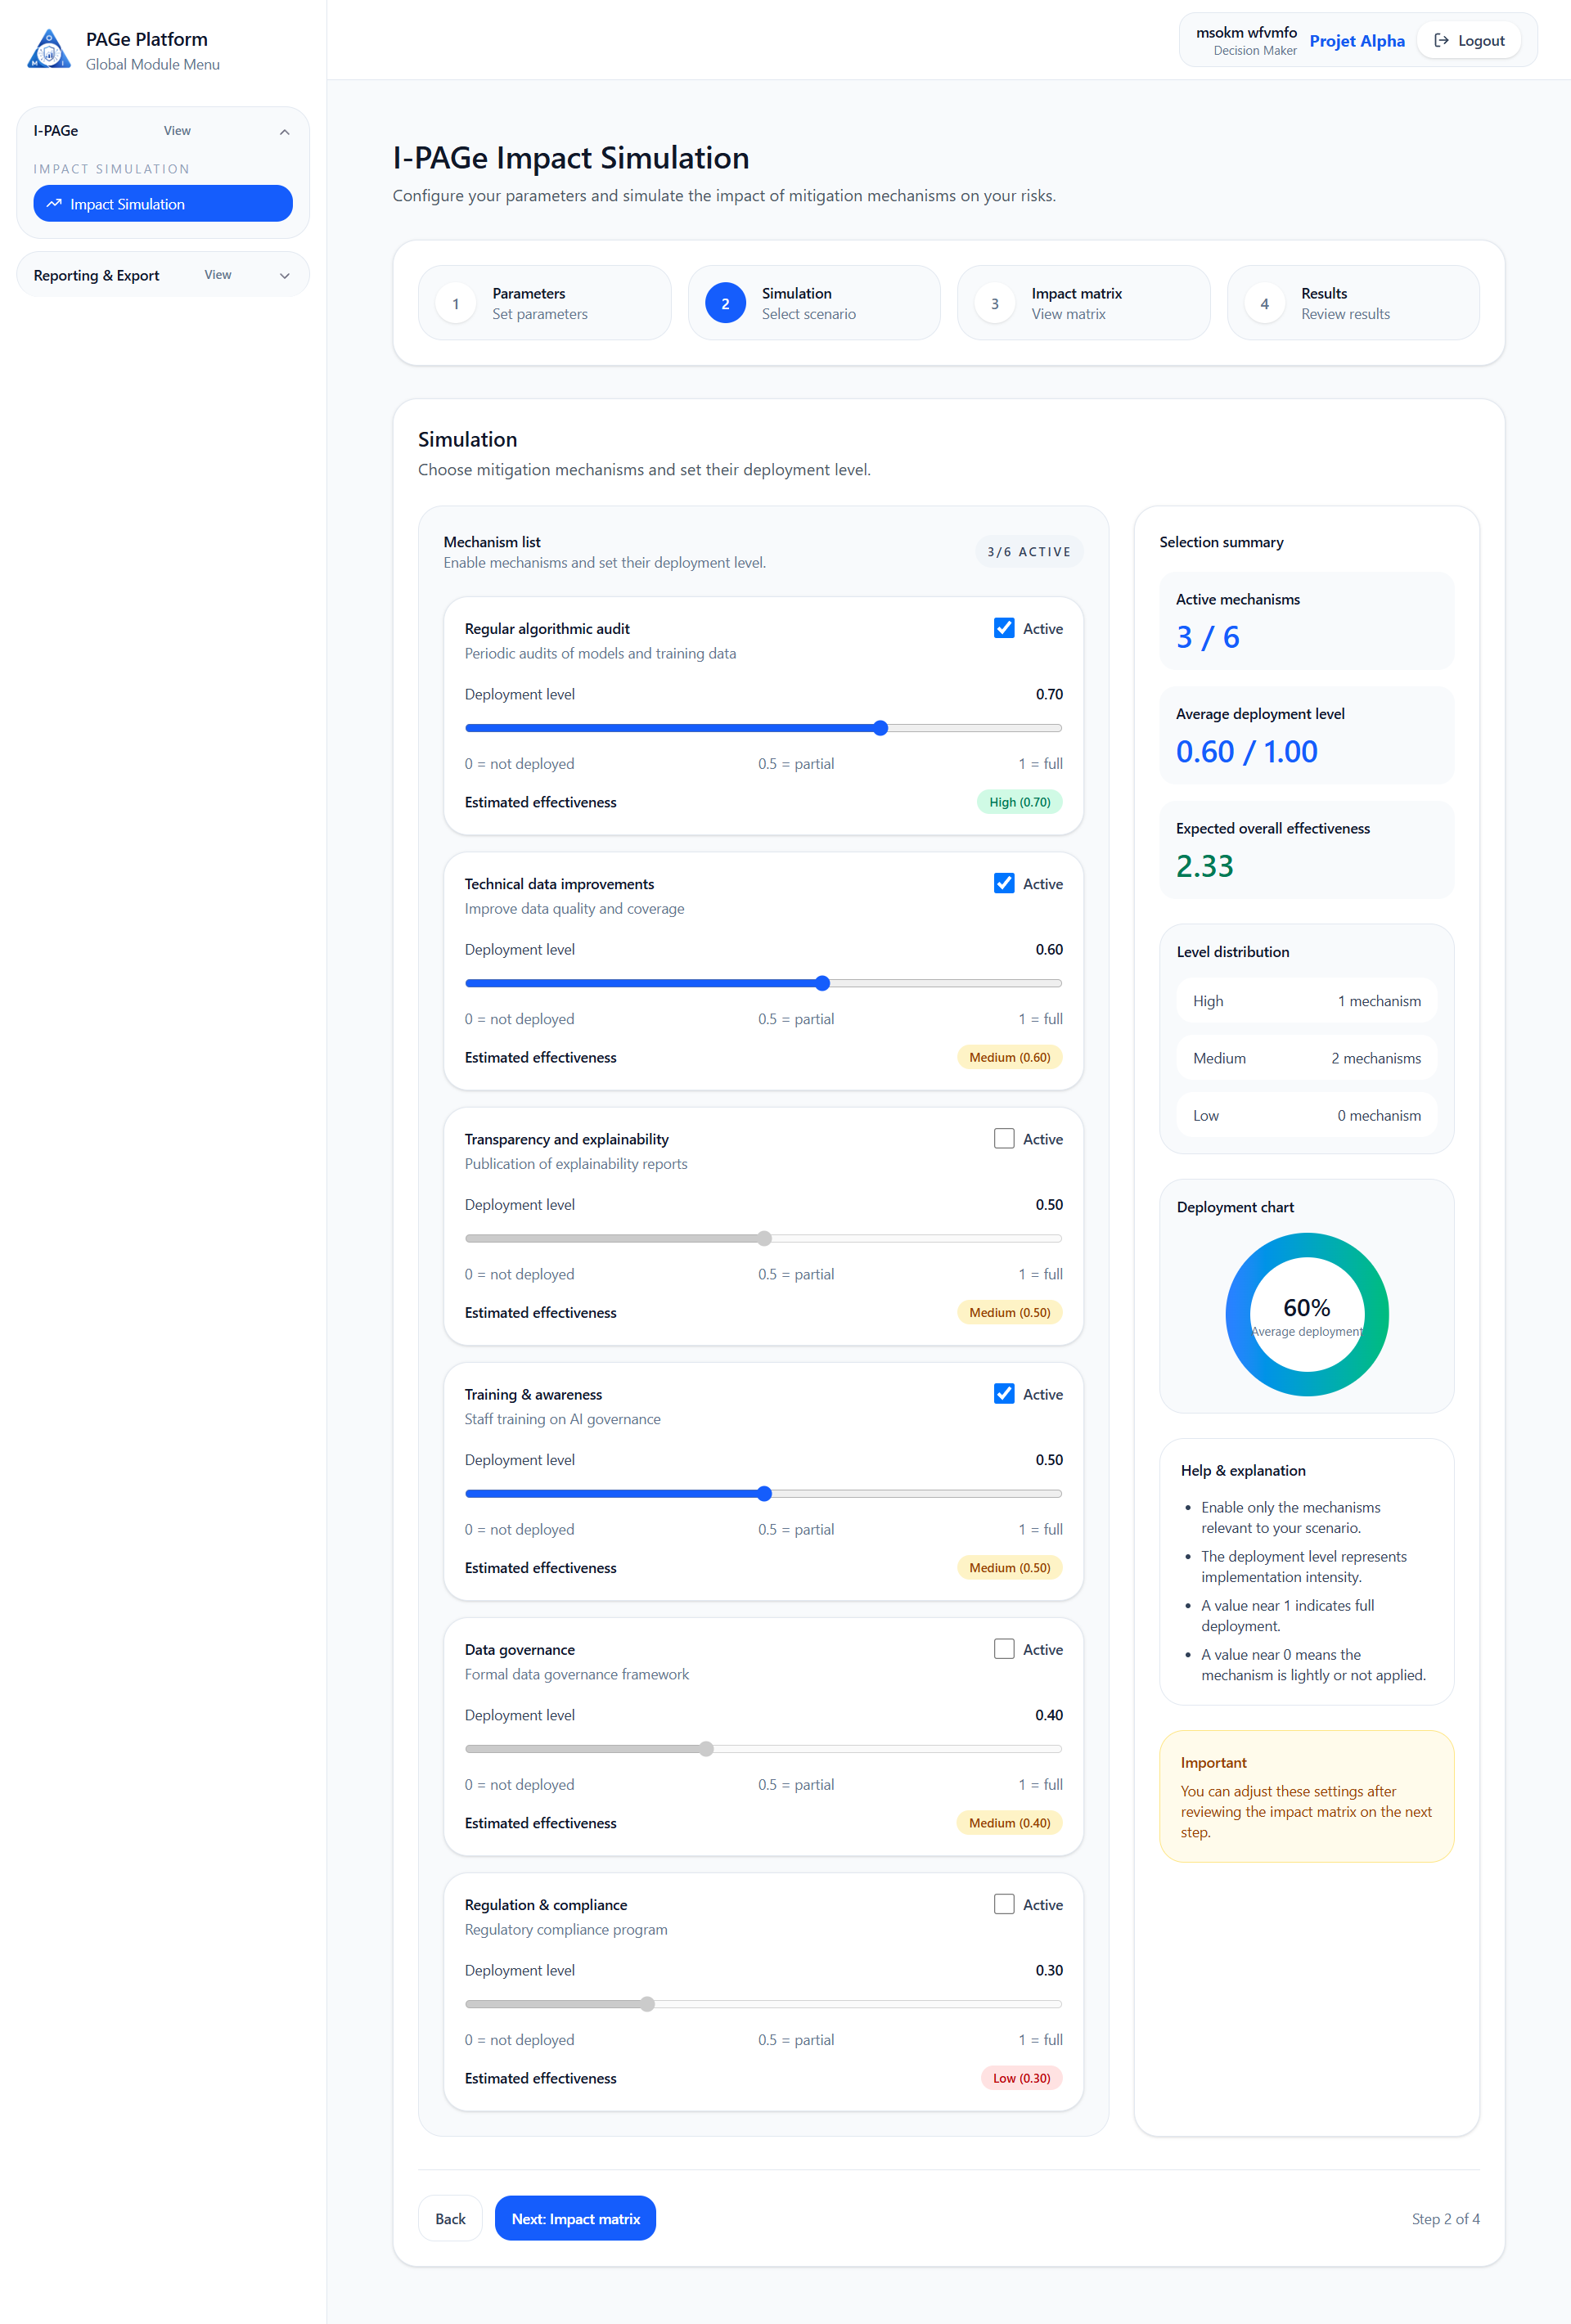
\includegraphics[width=0.8\textwidth]{Interfaces/Decision Maker/ONGLET2.png}
    \caption{Interface de Simulation}
\end{figure}
Cette interface, représentant la deuxième étape Simulation du module de simulation d'impact, permet au Décideur de choisir les mécanismes d’atténuation et de définir leur niveau de déploiement. Elle intègre un espace central pour activer les différents mécanismes du scénario et un panneau latéral regroupant le résumé de la sélection, notamment l'efficacité globale attendue. De plus, un graphique circulaire affiche le taux moyen de déploiement afin de guider l'utilisateur avant de passer à l'étape suivante de la matrice d'impact.
\begin{figure}[H]
    \centering
    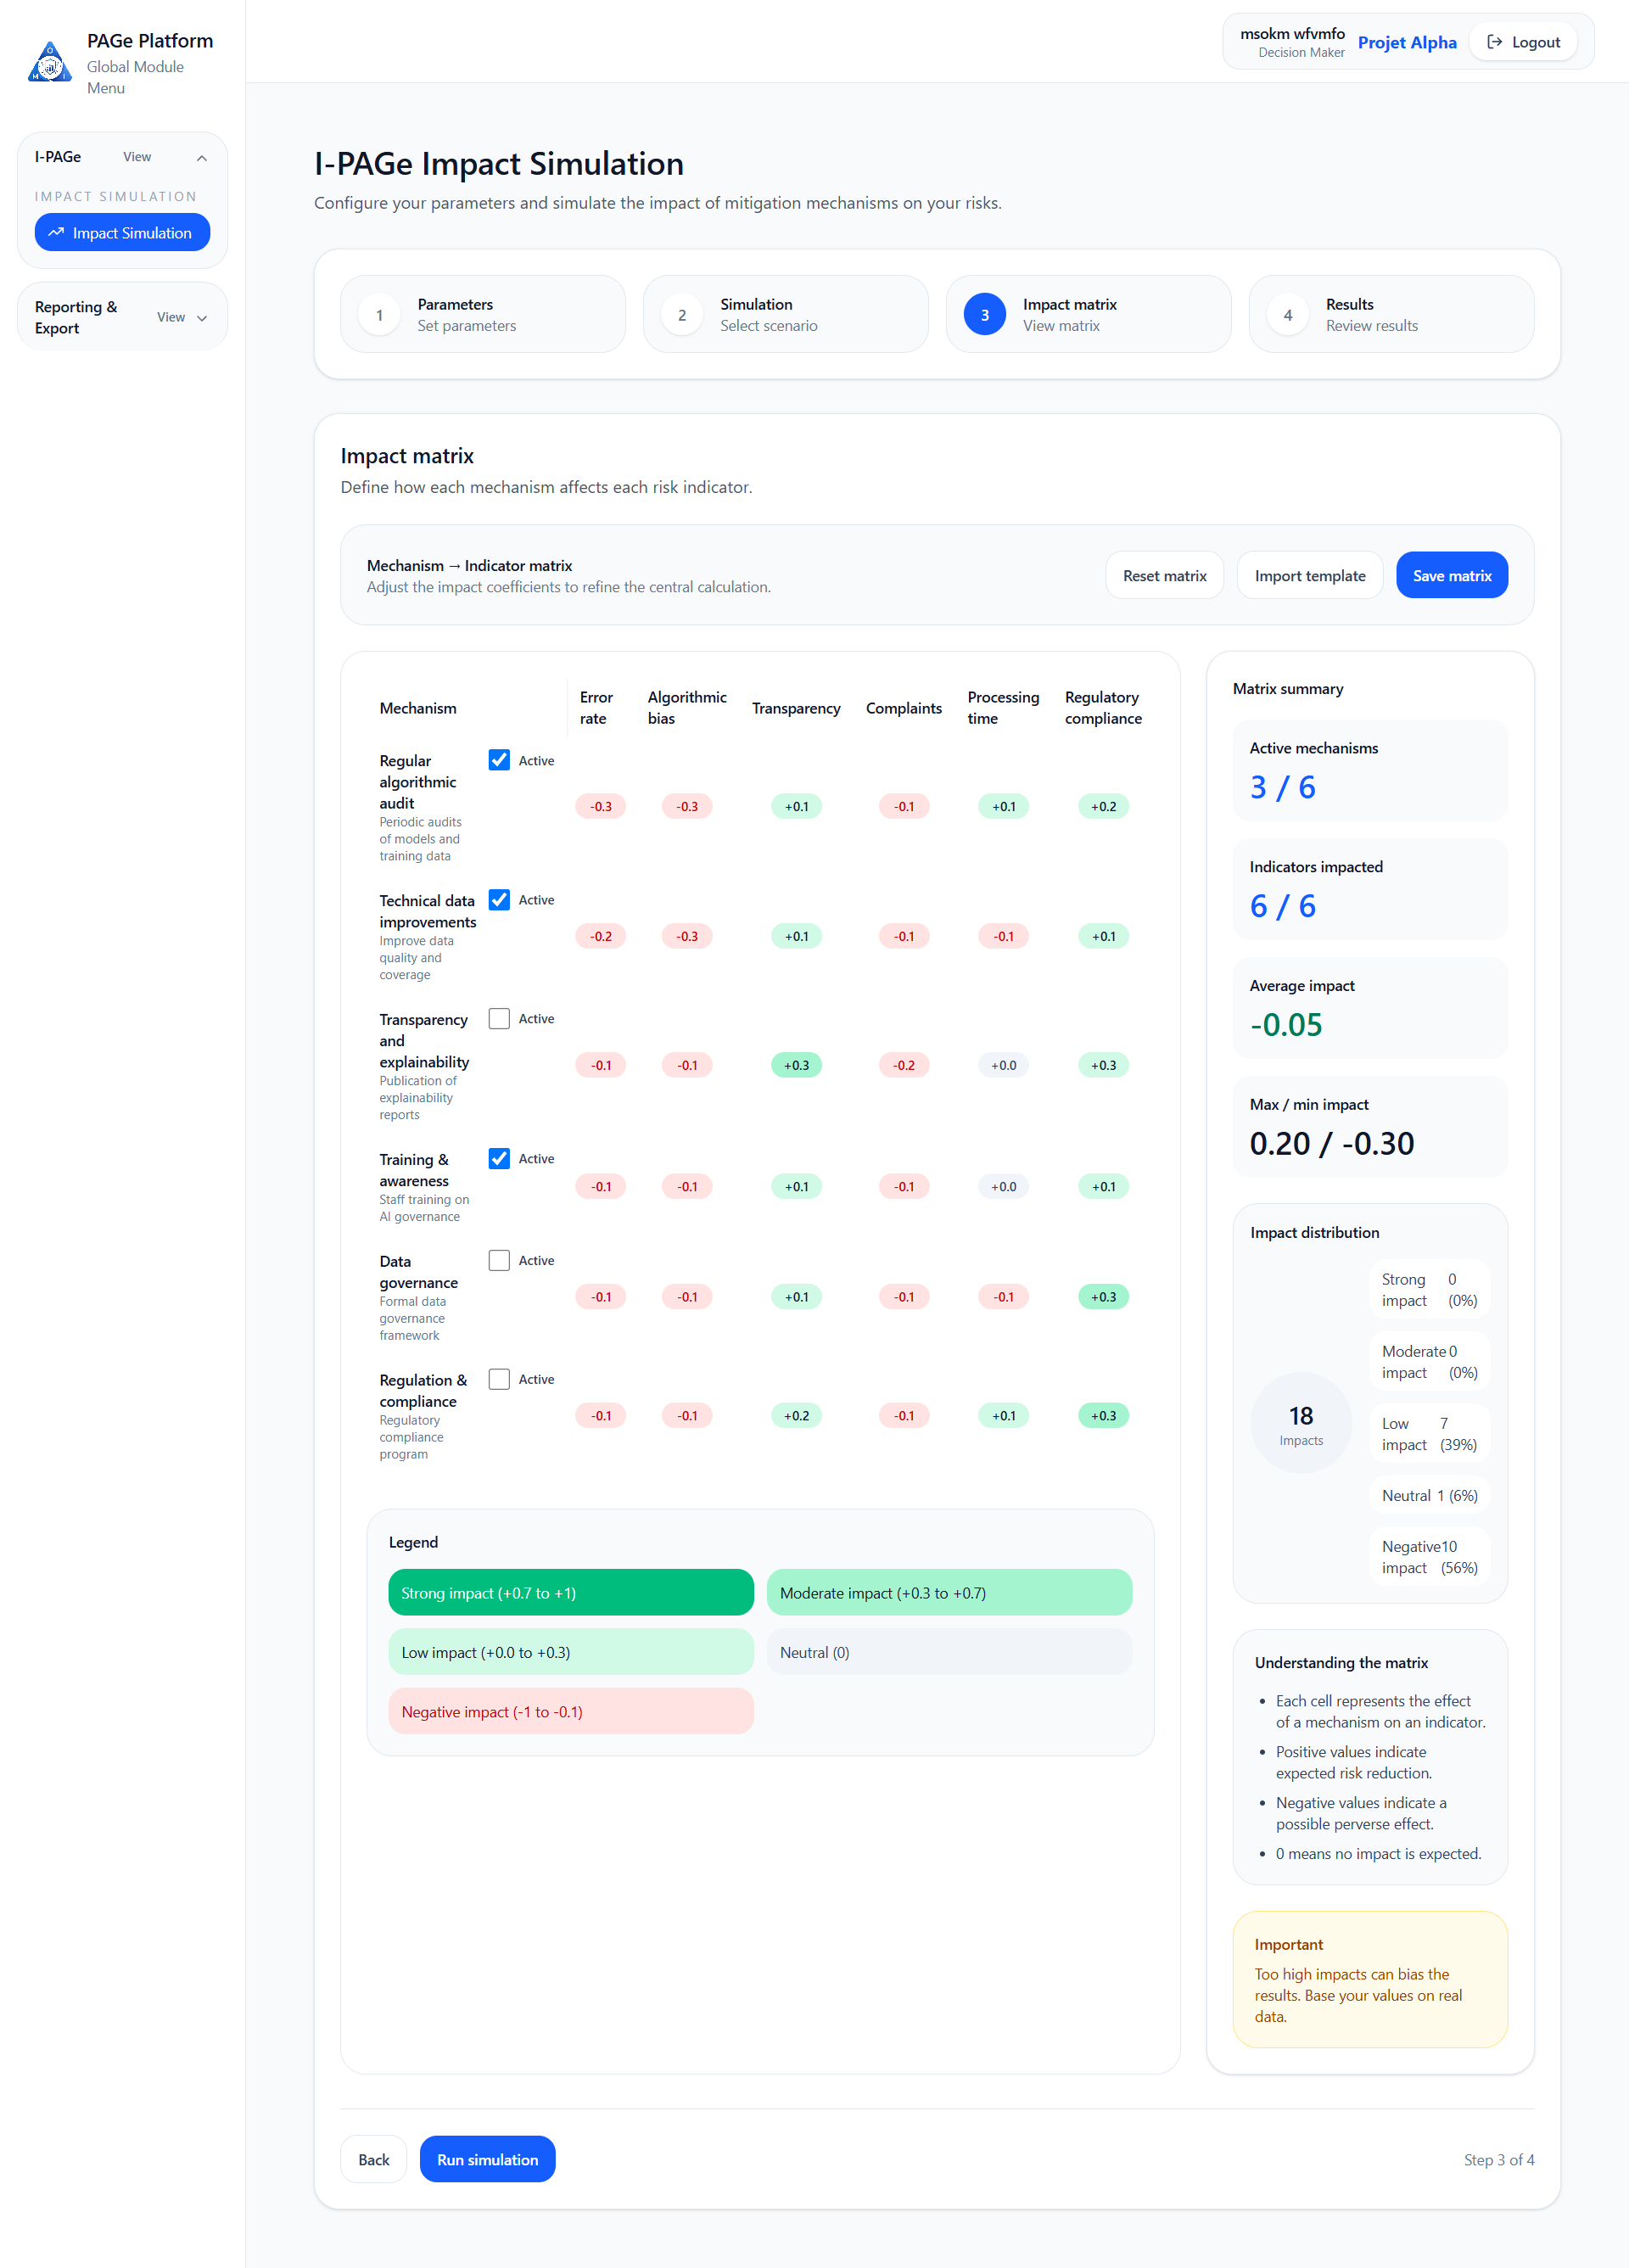
\includegraphics[width=0.8\textwidth]{Interfaces/Decision Maker/ONGLET3.png}
    \caption{Interface de matrice d'impact}
\end{figure}
Cette interface correspond à la troisième étape Impact matrix du processus, permettant au Décideur de définir et de visualiser l'effet de chaque mécanisme sur les indicateurs de risque. Elle présente un espace de configuration basé sur un code couleur (fort, modéré, faible ou négatif) pour ajuster précisément les coefficients d'impact du modèle.

\begin{figure}[H]
    \centering
    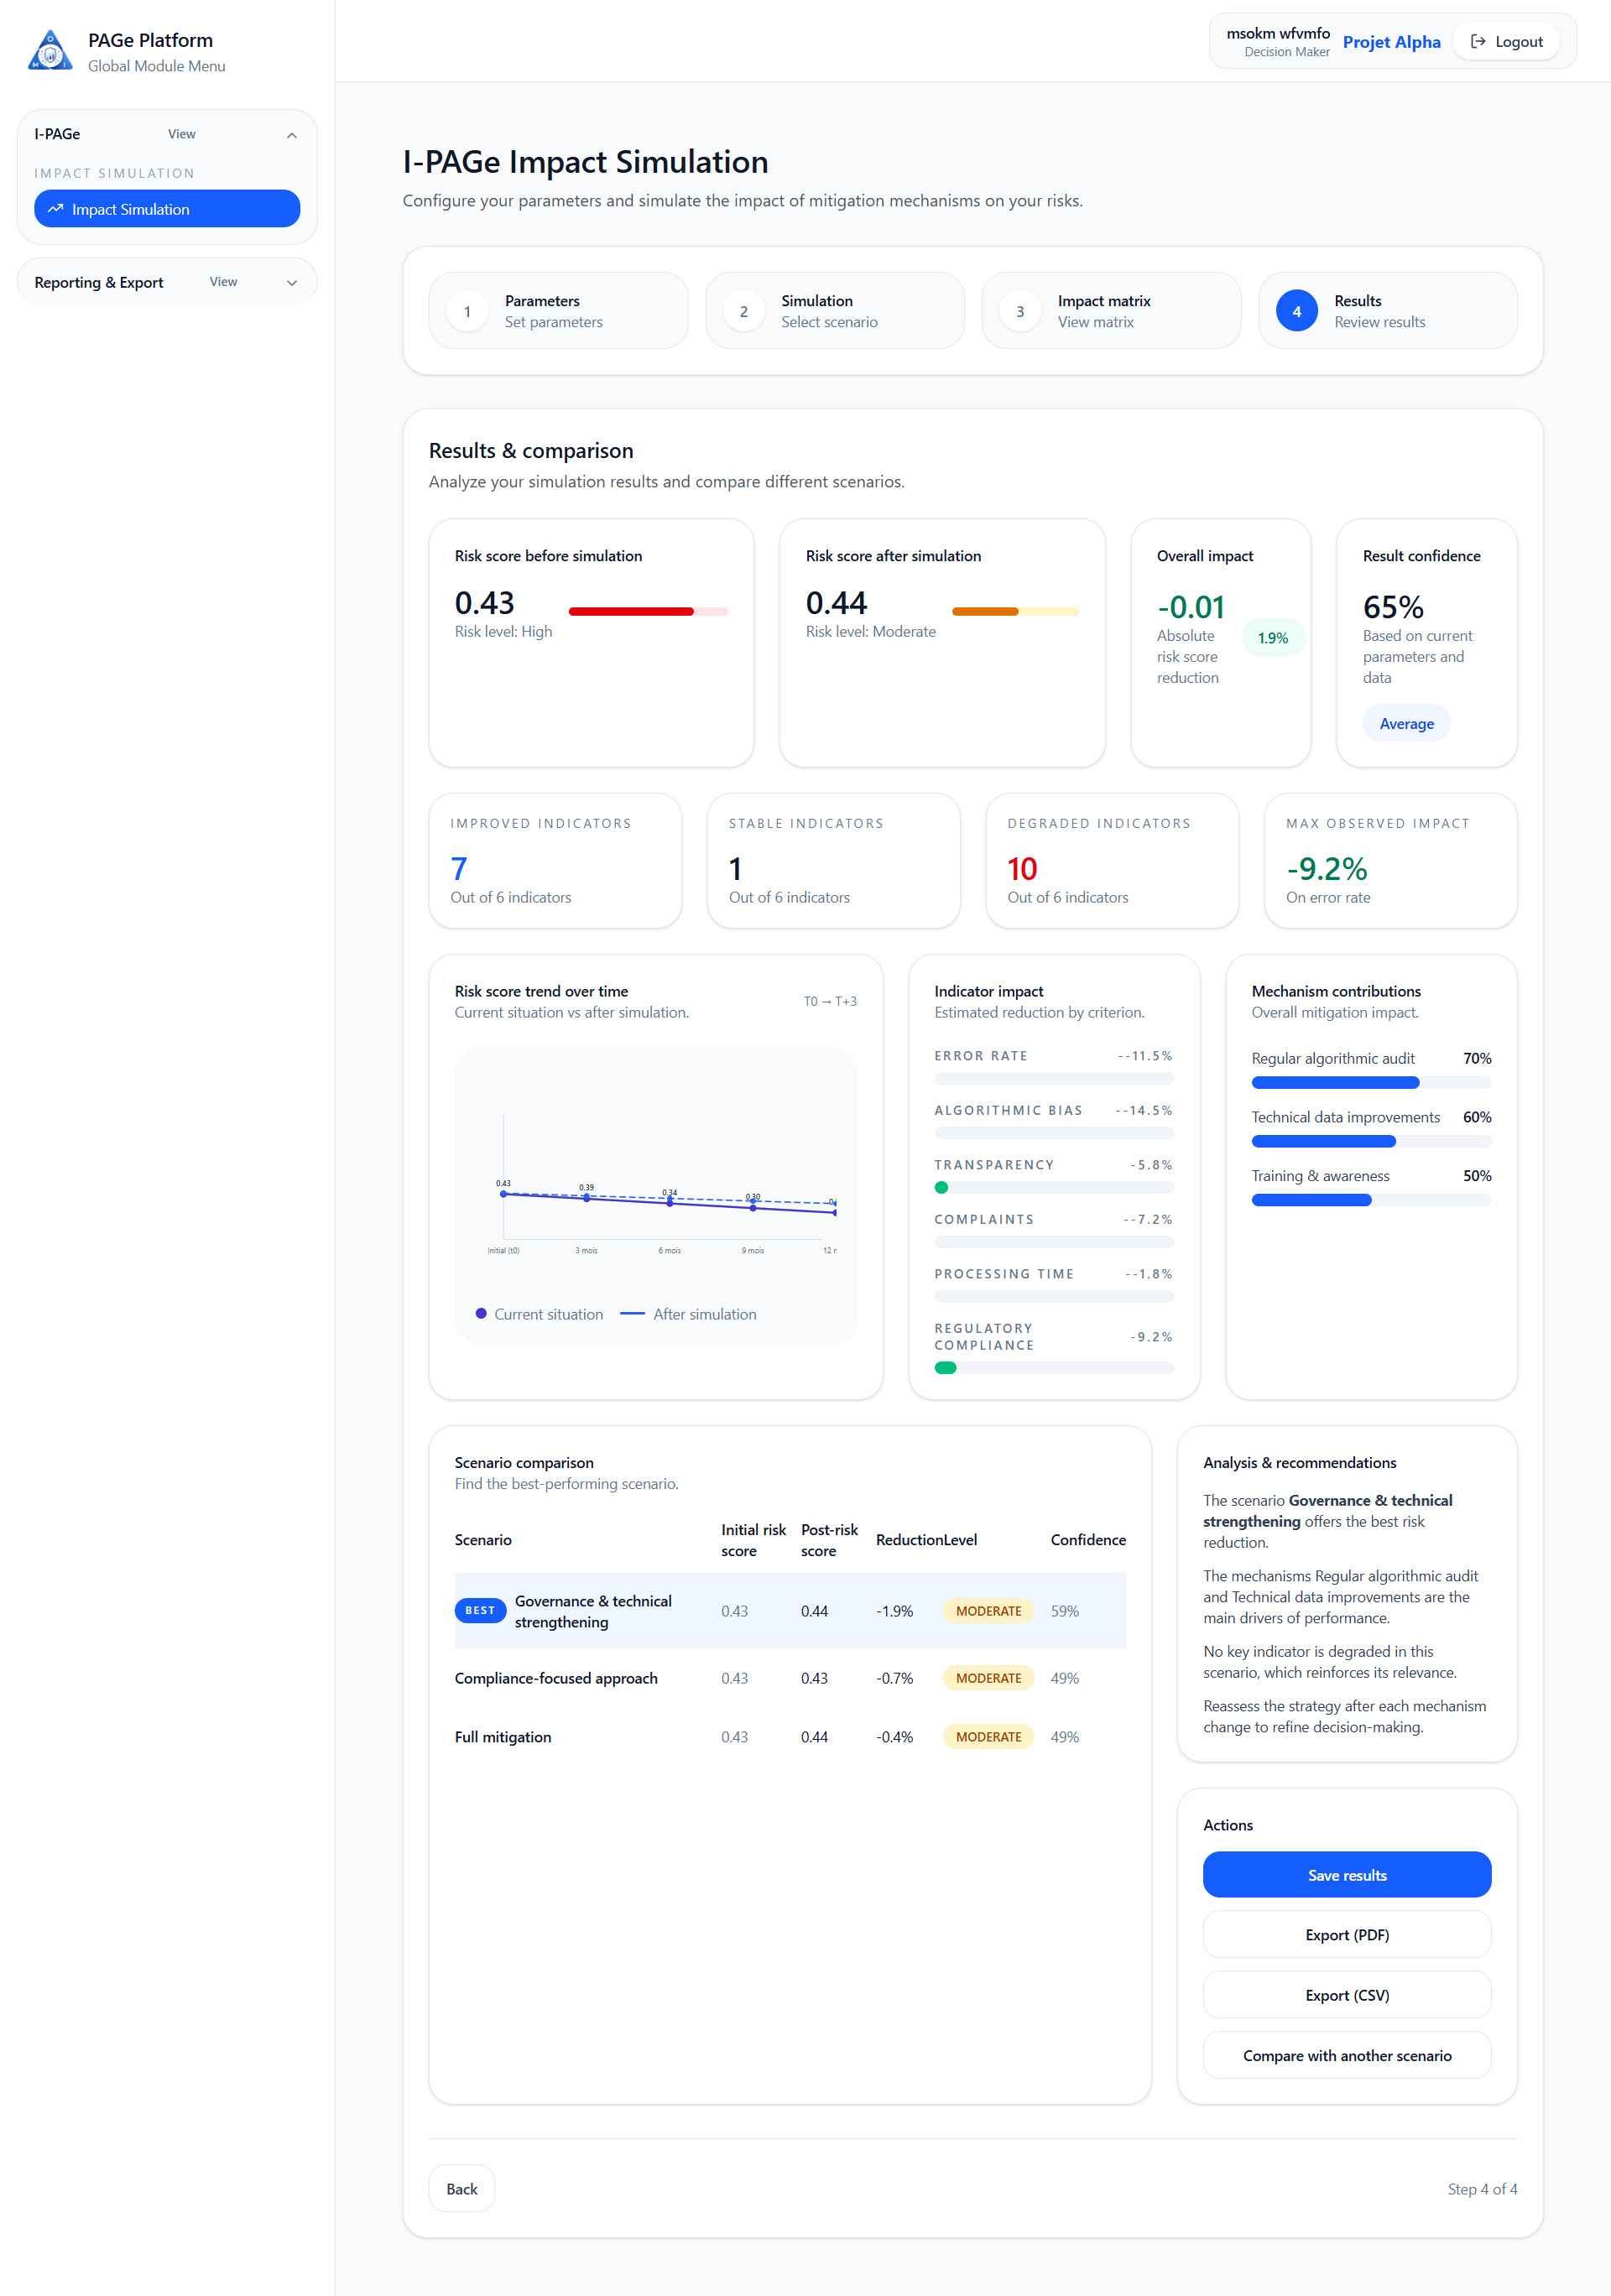
\includegraphics[width=0.8\textwidth]{Interfaces/Decision Maker/ONGLET4.png}
    \caption{Interface de matrice d'impact}
\end{figure}
L'interface Results \& comparison affiche les conclusions de la simulation d'impact pour le Décideur. Ce tableau de bord complet compare le score de risque avant et après simulation, tout en détaillant l'évolution des indicateurs (améliorés, stables ou dégradés) et les contributions de chaque mécanisme d'atténuation. Enfin, un outil de comparaison des scénarios et un bloc d'analyse automatique guident l'utilisateur dans sa prise de décision, avec des options pour sauvegarder ou exporter les rapports.
\subsubsection{Export les rapports}
\begin{figure}[H]
    \centering
    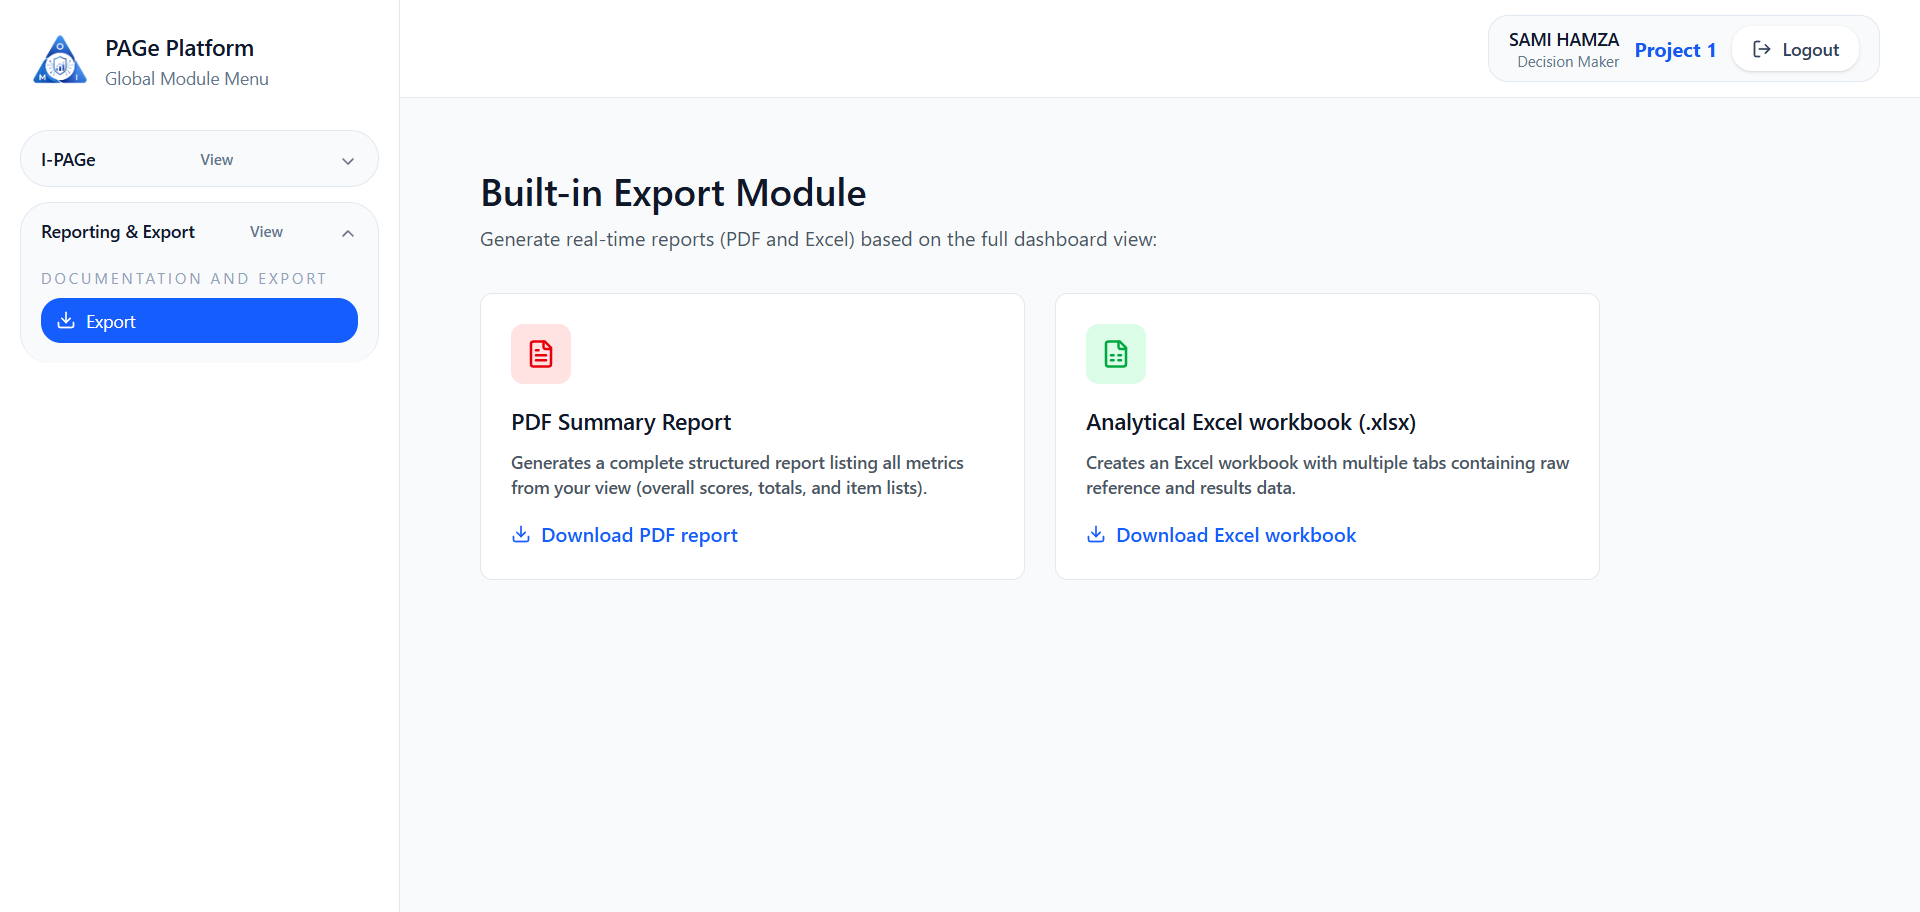
\includegraphics[width=0.8\textwidth]{Interfaces/Decision Maker/Export Data.png}
    \caption{Interface d'export les rapports}
\end{figure}
L'interface Export Data permet au Décideur de télécharger les synthèses de ses évaluations. Cet espace offre la possibilité de sélectionner un projet et une campagne spécifique afin de générer le rapport correspondant. À l'aide de boutons d'action épurés, l'utilisateur peut choisir d'exporter ses données et graphiques directement au format CSV ou au format PDF selon ses besoins.

\subsection{Les interfaces de l'Auditeur}
\subsubsection{Consultation des résultats}
\begin{figure}[H]
    \centering
    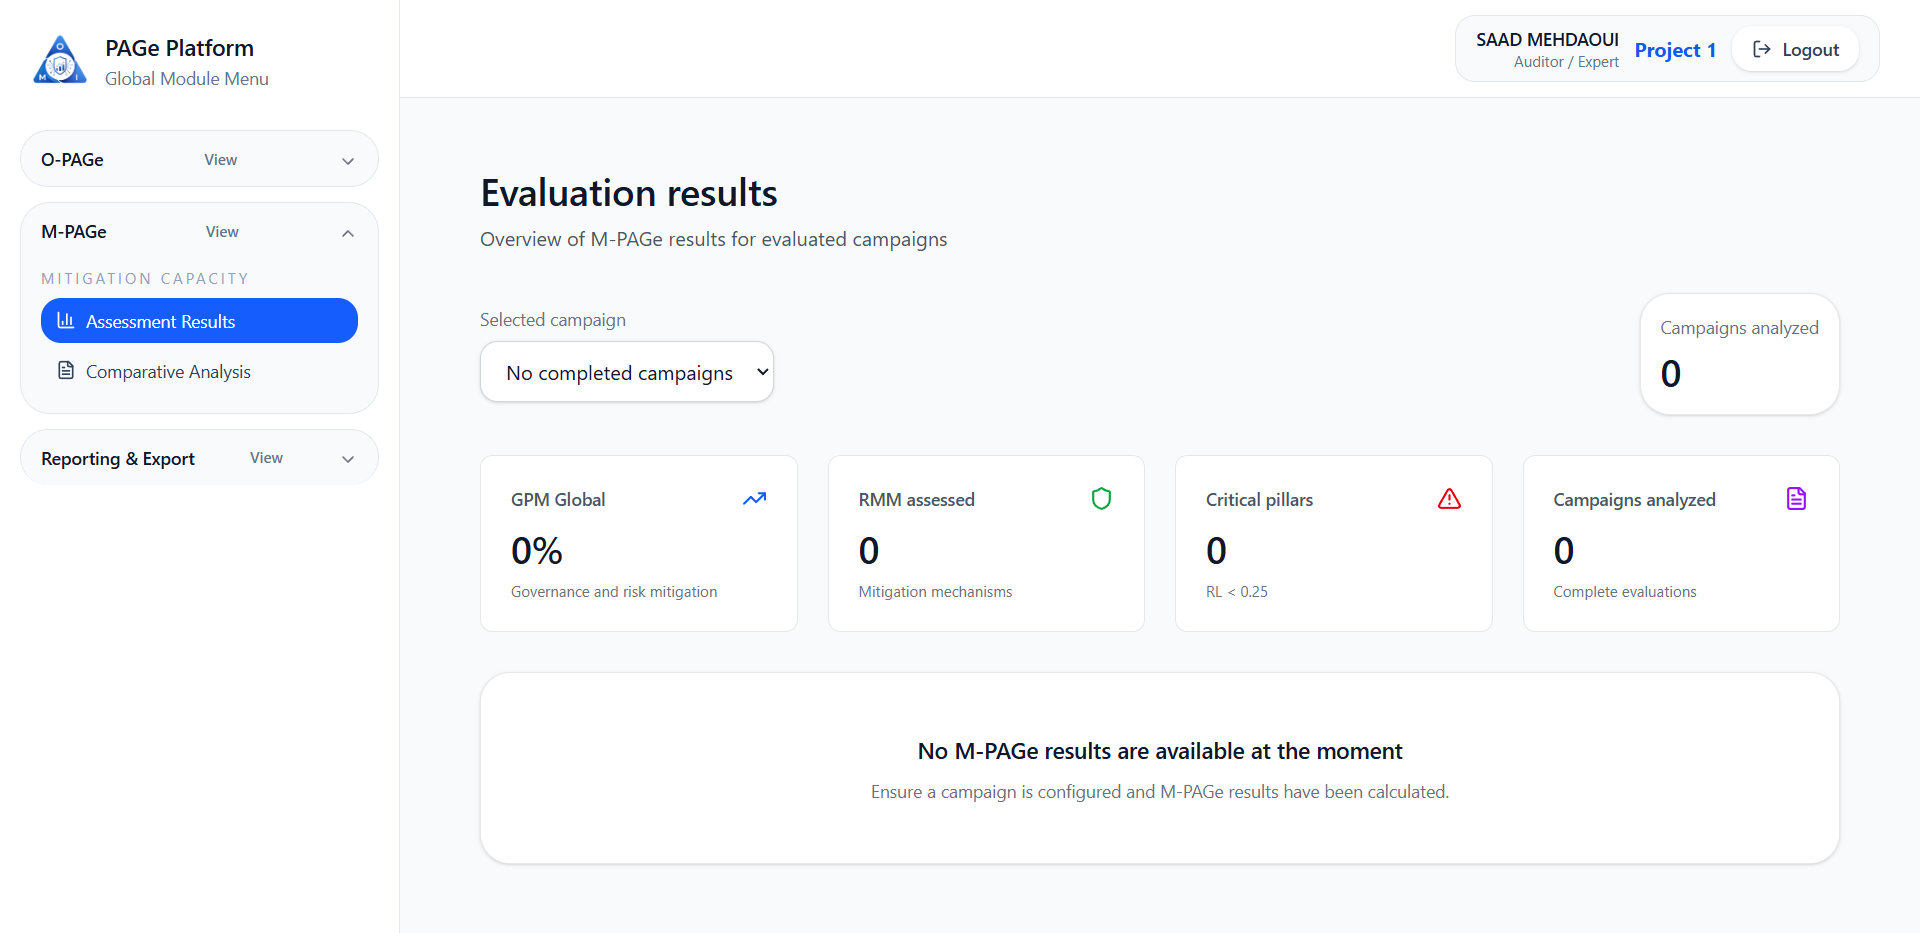
\includegraphics[width=0.8\textwidth]{Interfaces/Auditor/Evaluation Results.png}
    \caption{Interface de consultation les résultats}
\end{figure}
L'interface Evaluation results permet à l'Auditeur de consulter les résultats des campagnes d'évaluation. À l'aide d'un menu déroulant, l'utilisateur peut sélectionner une campagne spécifique afin d'afficher ses données de synthèse. Ce tableau de bord restitue alors des indicateurs de contrôle clés, tels que le score global de gouvernance (GPM Global), le nombre de mécanismes d'atténuation évalués (RMM assessed) ainsi que les piliers critiques du projet.

\subsubsection{Analyse des résultats}\begin{figure}[H]
    \centering
    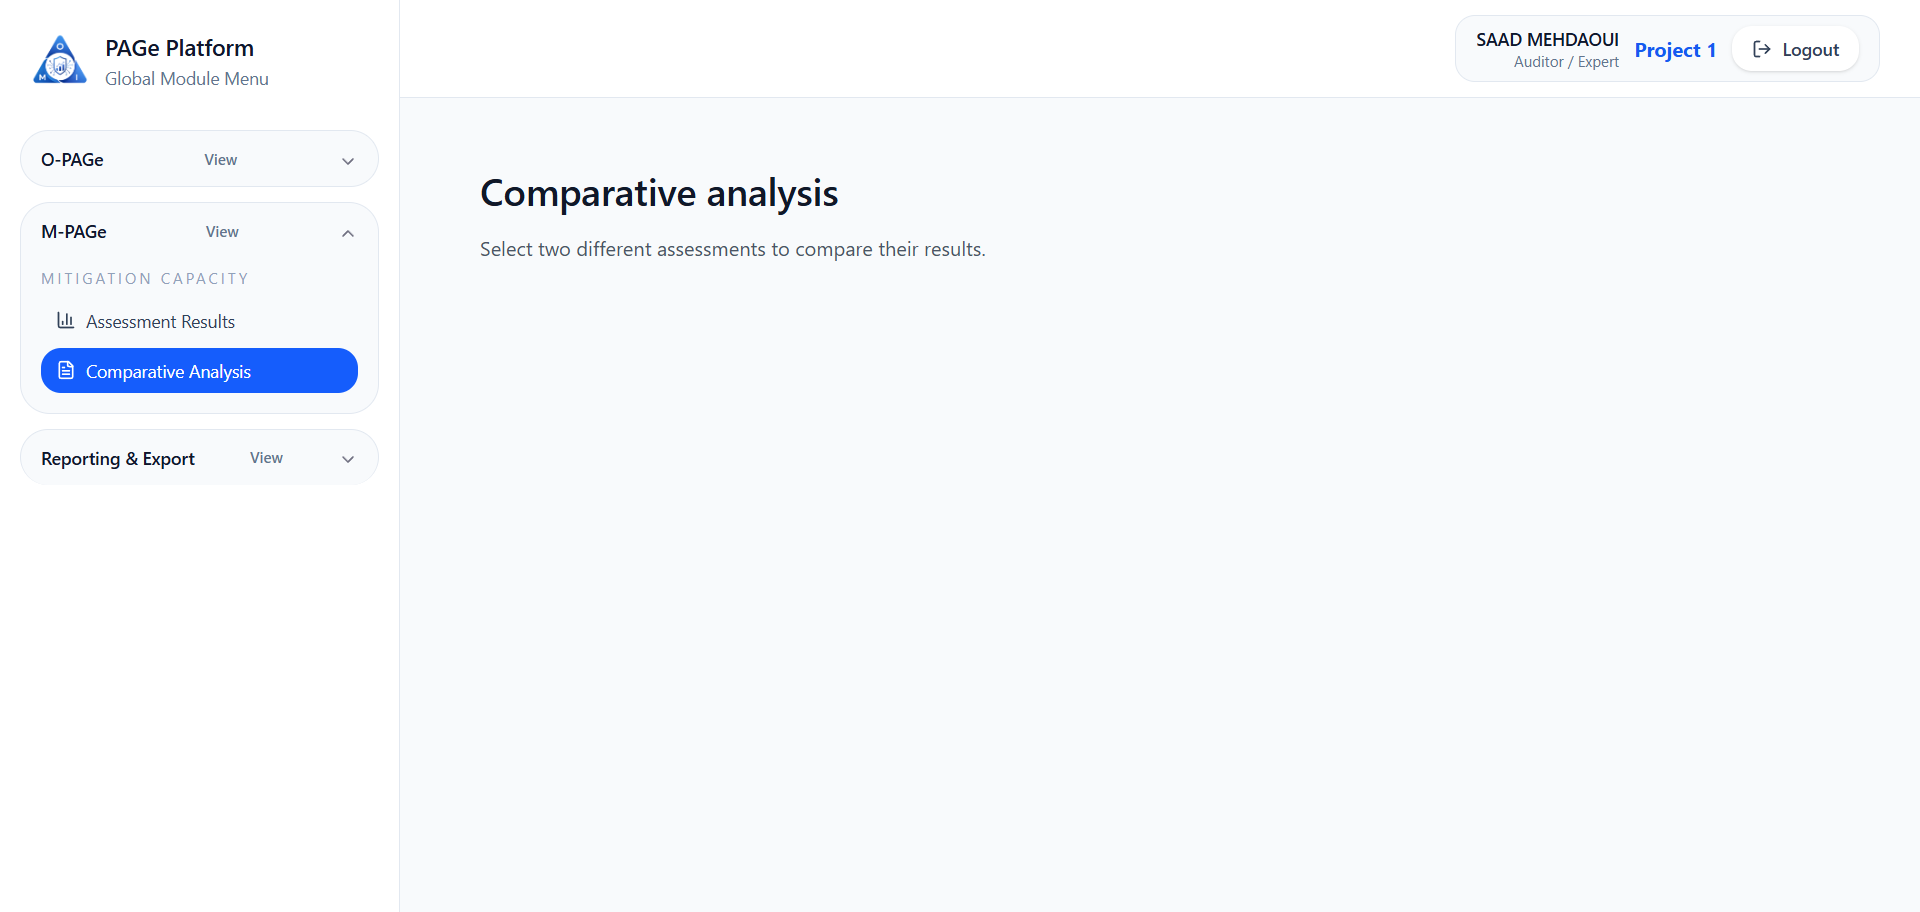
\includegraphics[width=0.8\textwidth]{Interfaces/Auditor/Comparative analysis.png}
    \caption{Interface d'analyse les résultats}
\end{figure}
L'interface Comparative analysis  permet à l'auditeur de confronter les données de la plateforme. Cet espace offre la possibilité de sélectionner deux évaluations distinctes afin de comparer directement leurs résultats côte à côte. Cet outil permet ainsi de mesurer l'évolution de la situation et d'évaluer l'impact des actions menées avant et après la mise en place de la mitigation.
\subsubsection{Consultation des risques et scores}\begin{figure}[H]
    \centering
    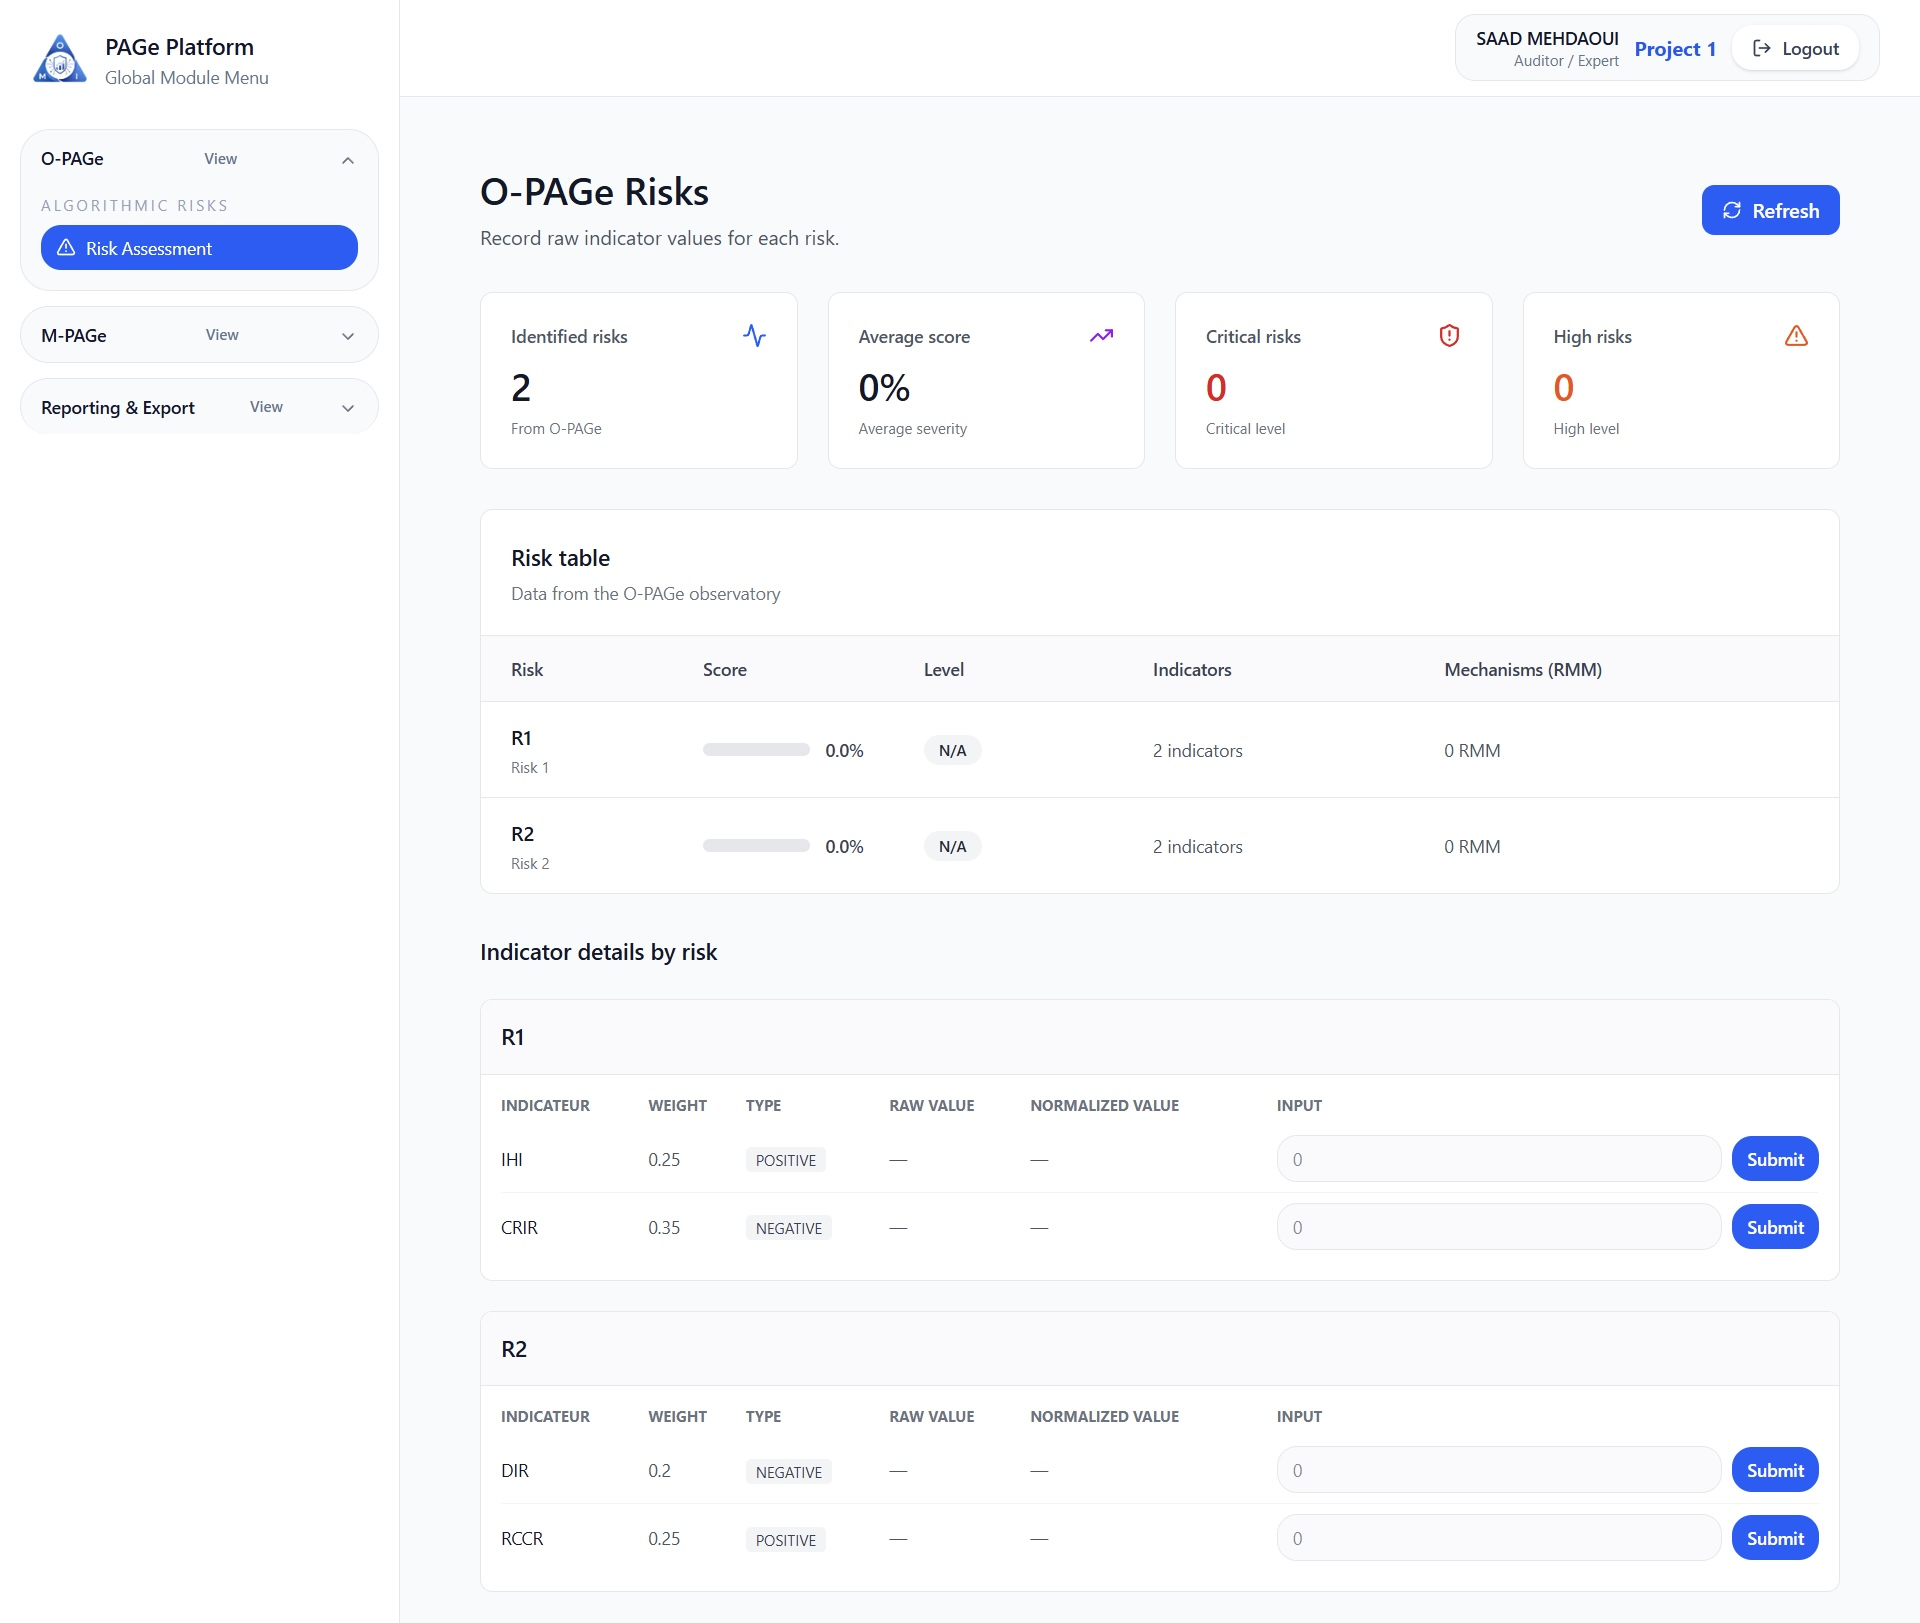
\includegraphics[width=0.8\textwidth]{Interfaces/Auditor/O-PAGe Risks.jpeg}
    \caption{Interface consultation des risques et scores}
\end{figure}
L'interface O-PAGe Risks offre à l'auditeur une vue d’ensemble analytique et consolidée des menaces identifiées. Elle présente des indicateurs de haut niveau tels que le score moyen de sévérité ou le nombre de risques critiques, complétés par un tableau de synthèse recensant les indicateurs rattachés et les mécanismes d'atténuation (RMM).


\section{Conclusion}

Ce chapitre a présenté la phase de réalisation de la plateforme PAGe, depuis le choix des outils et technologies jusqu'à la mise en œuvre concrète des différentes interfaces utilisateur. Nous avons détaillé l'environnement technique adopté, à savoir React avec Vite et Tailwind CSS pour le frontend, Django REST Framework pour le backend, PostgreSQL pour la persistance des données, et Docker pour la conteneurisation et le déploiement.

La présentation des interfaces a permis d'illustrer le fonctionnement des trois modules principaux de la plateforme : O-PAGe pour l'évaluation des risques algorithmiques via des indicateurs quantitatifs, M-PAGe pour la mesure de la maturité organisationnelle à travers des questionnaires structurés, et I-PAGe pour la simulation d'impact des mécanismes d'atténuation. Chaque rôle identifié lors de la phase de conception dispose d'un espace dédié, offrant des fonctionnalités adaptées à ses responsabilités.

L'ensemble des interfaces développées respecte les principes d'ergonomie et de clarté, avec des tableaux de bord synthétiques, des outils de comparaison avant/après, et des fonctionnalités d'export permettant aux différents acteurs de prendre des décisions éclairées en matière de gouvernance algorithmique.
